\section{The Z property implies Confluence}




  An ARS is defined as a pair composed of a set and binary operation
  over this set. Given an ARS $(A,R)$, where $A$ is a set, $R:A\times
  A$ and $a,b: A$, we write $a\ R\ b$ or $a\to_R b$ to denote that
  $(a,b)\in R$, and we say that $a$ $R$-reduces to $b$ in one step
  . The arrow notation will be prefered because it is more convenient
  for expressing reductions, so the reflexive transitive closure of a
  relation \coqdocvar{R}, written as $\tto_R$, is defined by the following
  inference rules: \begin{mathpar} \inferrule*[Right={$(refl)$}]{~}{a
  \tto_R a} \and \inferrule*[Right={$(rtrans)$}]{a\to_R b \and b
  \tto_R c}{a \tto_R c} \end{mathpar} \noindent where $a,b$ and $c$
  are universally quantified variables as one makes explicit in the
  corresponding Coq definition: \begin{coqdoccode}
\coqdocemptyline
\coqdocnoindent
\coqdockw{Inductive} \coqdef{ZtoConfl.refltrans}{refltrans}{\coqdocinductive{refltrans}} \{\coqdocvar{A}:\coqdockw{Type}\} (\coqdocvar{R}: \coqref{ZtoConfl.Rel}{\coqdocdefinition{Rel}} \coqdocvariable{A}) : \coqdocvar{A} \coqexternalref{::type scope:x '->' x}{http://coq.inria.fr/distrib/V8.11.0/stdlib//Coq.Init.Logic}{\coqdocnotation{\ensuremath{\rightarrow}}} \coqdocvar{A} \coqexternalref{::type scope:x '->' x}{http://coq.inria.fr/distrib/V8.11.0/stdlib//Coq.Init.Logic}{\coqdocnotation{\ensuremath{\rightarrow}}} \coqdockw{Prop} :=\coqdoceol
\coqdocnoindent
\ensuremath{|} \coqdef{ZtoConfl.refl}{refl}{\coqdocconstructor{refl}}: \coqdockw{\ensuremath{\forall}} \coqdocvar{a}, (\coqref{ZtoConfl.refltrans}{\coqdocinductive{refltrans}} \coqdocvariable{R}) \coqdocvariable{a} \coqdocvariable{a}\coqdoceol
\coqdocnoindent
\ensuremath{|} \coqdef{ZtoConfl.rtrans}{rtrans}{\coqdocconstructor{rtrans}}: \coqdockw{\ensuremath{\forall}} \coqdocvar{a} \coqdocvar{b} \coqdocvar{c}, \coqdocvariable{R} \coqdocvariable{a} \coqdocvariable{b} \coqexternalref{::type scope:x '->' x}{http://coq.inria.fr/distrib/V8.11.0/stdlib//Coq.Init.Logic}{\coqdocnotation{\ensuremath{\rightarrow}}} \coqref{ZtoConfl.refltrans}{\coqdocinductive{refltrans}} \coqdocvariable{R} \coqdocvariable{b} \coqdocvariable{c} \coqexternalref{::type scope:x '->' x}{http://coq.inria.fr/distrib/V8.11.0/stdlib//Coq.Init.Logic}{\coqdocnotation{\ensuremath{\rightarrow}}} \coqref{ZtoConfl.refltrans}{\coqdocinductive{refltrans}} \coqdocvariable{R} \coqdocvariable{a} \coqdocvariable{c}.\coqdoceol
\coqdocemptyline
\end{coqdoccode}
The rule names (\coqdocvar{refl}) and (\coqdocvar{rtrans}) are called \textit{constructors}
in the Coq definition. The first constructor states the reflexivity of
$\tto_R$, while \coqdocvar{rtrans} extends the reflexive transitive closure of
\coqdocvar{R} if one has at least a one-step reduction. As a first example,
let's have a look at the proof of transitivity of $\tto_R$:


\begin{lemma} Let $\to_R$ be a binary relation over a set $A$. For all
$t,u,v \in A$, if $t \tto_R u$ and $u \tto_R v$ then $t \tto_R v$.
\end{lemma}


 Although its simplicity, it will help us to explain the way we will
relate English annotations with the proof steps. The corresponding
lemma in Coq, named \coqdocvar{refltrans\_composition}, is stated as follows: \begin{coqdoccode}
\coqdocemptyline
\coqdocnoindent
\coqdockw{Lemma} \coqdef{ZtoConfl.refltrans composition}{refltrans\_composition}{\coqdoclemma{refltrans\_composition}} \{\coqdocvar{A}\} (\coqdocvar{R}: \coqref{ZtoConfl.Rel}{\coqdocdefinition{Rel}} \coqdocvariable{A}):\coqdoceol
\coqdocindent{1.00em}
\coqdockw{\ensuremath{\forall}} \coqdocvar{t} \coqdocvar{u} \coqdocvar{v}, \coqref{ZtoConfl.refltrans}{\coqdocinductive{refltrans}} \coqdocvariable{R} \coqdocvariable{t} \coqdocvariable{u} \coqexternalref{::type scope:x '->' x}{http://coq.inria.fr/distrib/V8.11.0/stdlib//Coq.Init.Logic}{\coqdocnotation{\ensuremath{\rightarrow}}} \coqref{ZtoConfl.refltrans}{\coqdocinductive{refltrans}} \coqdocvariable{R} \coqdocvariable{u} \coqdocvariable{v} \coqexternalref{::type scope:x '->' x}{http://coq.inria.fr/distrib/V8.11.0/stdlib//Coq.Init.Logic}{\coqdocnotation{\ensuremath{\rightarrow}}} \coqref{ZtoConfl.refltrans}{\coqdocinductive{refltrans}} \coqdocvariable{R} \coqdocvariable{t} \coqdocvariable{v}.\coqdoceol
\coqdocemptyline
\end{coqdoccode}
This work is not a Coq tutorial, but our idea is that it should
also be readable for those unfamiliar with the Coq proof Assistant. In
addition, this paper is built directly from a Coq proof script, which
means that we are forced to present the ideas and the results in a
more organized and systematic way that is not necessarily the more
pedagogical one. In this way, we decided to comment the proof steps
giving the general idea of what they do. It is done in such a way that
both parts (informal and formal) are mostly independent, and those not
interested in the Coq part can focus just on the informal
part. Firstly, notice that proofs are written between the reserved
words \coqdockw{Proof} and \coqdockw{Qed}. Each proof command finishes with a dot, and
proofs can be structured with bullets. \begin{coqdoccode}
\coqdocemptyline
\coqdocnoindent
\coqdockw{Proof}.\coqdoceol
\coqdocindent{1.00em}
\coqdoctac{intros} \coqdocvar{t} \coqdocvar{u} \coqdocvar{v} \coqdocvar{H1} \coqdocvar{H2}. \end{coqdoccode}
Let \coqdocvar{t},\coqdocvar{u} and \coqdocvar{v} be elements of type \coqdocvar{A}
      (or be elements of the set \coqdocvar{A}), and assume that $t \tto_R u$
      (name this assumption \coqdocvar{H1}) and $u\tto_R v$ (assumption
      \coqdocvar{H2}). The corresponding proof context shows the hypothesis and
      the goal separated by a horizontal line: \newline


      \begin{figure}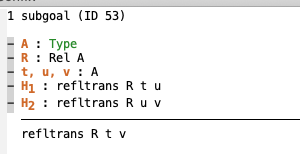
\includegraphics[scale=0.6]{fig1.png}
      \caption{Transitivity of refltrans}
      \label{fig:trans}\end{figure} \begin{coqdoccode}
\coqdocemptyline
\coqdocindent{1.00em}
\coqdoctac{induction} \coqdocvar{H1}. \end{coqdoccode}
The proof proceeds by induction on the hypothesis
      \coqdocvar{H1}, i.e. induction on $t \tto_R u$. The structure of the proof
      context models the induction hypothesis, and this fact will be
      essential to build the inductive proof of the next theorem. As
      shown in Figure \ref{fig:trans}, \coqdocvar{H2} is the sole hypothesis
      different from \coqdocvar{H1}, and hence the induction hypothesis will
      subsume \coqdocvar{H2}. \begin{coqdoccode}
\coqdocemptyline
\coqdocindent{1.00em}
- \coqdoctac{assumption}. \end{coqdoccode}
The first case is when $t \tto_R u$ is generated
      by the constructor $refl$, which is an axiom and hence we are
      done. \begin{coqdoccode}
\coqdocemptyline
\coqdocindent{1.00em}
- \coqdoctac{apply} \coqref{ZtoConfl.rtrans}{\coqdocconstructor{rtrans}} \coqdockw{with} \coqdocvar{b}. \end{coqdoccode}
The second case, i.e. the recursive case
      is more interesting because $t \tto_R u$ is now generated by
      $(rtrans)$. This means that there exists an element, say $b$,
      such that $t \to_R b$ and $b \tto_R u$. Therefore, in order to
      prove that $t \tto_R v$, we can apply the rule \coqdocvar{rtrans} taking
      \coqdocvar{b} as the intermediary term, and we have two subcases to
      prove: \begin{coqdoccode}
\coqdocemptyline
\coqdocindent{2.00em}
+ \coqdoctac{assumption}. \end{coqdoccode}
In the first case we need to prove that $t \to_R
    b$, which we have as hypothesis. \begin{coqdoccode}
\coqdocemptyline
\coqdocindent{2.00em}
+ \coqdoctac{apply} \coqdocvar{IHrefltrans}; \coqdoctac{assumption}. \end{coqdoccode}
In the second case, we prove
    that $b \tto_R v$ by the induction hypothesis $u \tto_R v \to b
    \tto_R v$, where $u\tto_R v$ is the hypothesis \coqdocvar{H2}. The proof of
    the recursive case may be better visualized by the corresponding
    deduction tree: {\scriptsize \begin{mathpar}
    \inferrule*[Right=MP]{\inferrule*[Right=MP]{\inferrule*[Right={
    $rtrans$}]{~}{\inferrule*[Right={$(\forall_e)$}]{\forall x\ y\ z,
    x\to_R y \to y\tto_R z \to x\tto_R z}{a\to_R b \to b\tto_R v \to
    a\tto_R v}} \and \inferrule*[Right={H}]{~}{a\to_R b}}{ b\tto_R v
    \to a\tto_R v} \and \inferrule*[Right=MP]{\inferrule*[Right={
    $IH$}]{~}{c\tto_R v \to b\tto_R v} \and
    \inferrule*[Right={H2}]{~}{c\tto_R v}}{b\tto_R v}}{a\tto_R v}
    \end{mathpar}} \begin{coqdoccode}
\coqdocnoindent
\coqdockw{Qed}.\coqdoceol
\coqdocemptyline
\end{coqdoccode}
This example is interesting because it shows how Coq works, how
tactics correspond in general to several steps of natural deduction
rules, and how proofs can be structured with bullets. \begin{coqdoccode}
\coqdocemptyline
\coqdocemptyline
\end{coqdoccode}
The reflexive transitive closure of a relation is used to define
    the notion of confluence: no matter how the reduction is done, the
    result will always be the same. In other words, every divergence
    is joinable as stated by the following diagram:


    $\begin{tabular}{c} \xymatrix{ & a \ar@{->>}[dl] \ar@{->>}[dr] &
    \\ b \ar@{.>>}[dr] & & c \ar@{.>>}[dl] \\ & d & } \end{tabular}$


    Therefore, if an expression $a$ can be reduced in two different
    ways to the expressions $b$ and $c$, then there exists an
    expression $d$ such that both $b$ and $c$ reduces to $d$. The
    existential quantification is expressed by the dotted lines in the
    diagram. This notion is defined in the Coq system as follows: \begin{coqdoccode}
\coqdocemptyline
\coqdocnoindent
\coqdockw{Definition} \coqdef{ZtoConfl.Confl}{Confl}{\coqdocdefinition{Confl}} \{\coqdocvar{A}:\coqdockw{Type}\} (\coqdocvar{R}: \coqref{ZtoConfl.Rel}{\coqdocdefinition{Rel}} \coqdocvariable{A}) := \coqdockw{\ensuremath{\forall}} \coqdocvar{a} \coqdocvar{b} \coqdocvar{c}, (\coqref{ZtoConfl.refltrans}{\coqdocinductive{refltrans}} \coqdocvariable{R}) \coqdocvariable{a} \coqdocvariable{b} \coqexternalref{::type scope:x '->' x}{http://coq.inria.fr/distrib/V8.11.0/stdlib//Coq.Init.Logic}{\coqdocnotation{\ensuremath{\rightarrow}}} (\coqref{ZtoConfl.refltrans}{\coqdocinductive{refltrans}} \coqdocvariable{R}) \coqdocvariable{a} \coqdocvariable{c} \coqexternalref{::type scope:x '->' x}{http://coq.inria.fr/distrib/V8.11.0/stdlib//Coq.Init.Logic}{\coqdocnotation{\ensuremath{\rightarrow}}} \coqexternalref{::type scope:x '->' x}{http://coq.inria.fr/distrib/V8.11.0/stdlib//Coq.Init.Logic}{\coqdocnotation{(}}\coqexternalref{::type scope:'exists' x '..' x ',' x}{http://coq.inria.fr/distrib/V8.11.0/stdlib//Coq.Init.Logic}{\coqdocnotation{\ensuremath{\exists}}} \coqdocvar{d}\coqexternalref{::type scope:'exists' x '..' x ',' x}{http://coq.inria.fr/distrib/V8.11.0/stdlib//Coq.Init.Logic}{\coqdocnotation{,}} (\coqref{ZtoConfl.refltrans}{\coqdocinductive{refltrans}} \coqdocvariable{R}) \coqdocvariable{b} \coqdocvariable{d} \coqexternalref{::type scope:x '/x5C' x}{http://coq.inria.fr/distrib/V8.11.0/stdlib//Coq.Init.Logic}{\coqdocnotation{\ensuremath{\land}}} (\coqref{ZtoConfl.refltrans}{\coqdocinductive{refltrans}} \coqdocvariable{R}) \coqdocvariable{c} \coqdocvariable{d}\coqexternalref{::type scope:x '->' x}{http://coq.inria.fr/distrib/V8.11.0/stdlib//Coq.Init.Logic}{\coqdocnotation{)}}.\coqdoceol
\coqdocemptyline
\end{coqdoccode}
In \cite{ZPropertyDraft}, V. van Oostrom gives a suficient
    condition for an ARS to be confluent, known as the \textit{Z Property}:


    \begin{definition} Let $(A,\to_R)$ be an abstract rewriting system
      (ARS). The system $(A,\to_R)$ has the Z property, if there exists
      a map $f:A \to A$ such that the following diagram holds:
    
      \[ \xymatrix{ a \ar[r]_R & b \ar@{.>>}[dl]^R\\ f(a) \ar@{.>>}[r]_R &
      f(b) \\ } \] \end{definition}


The corresponding Coq definition is given as: \begin{coqdoccode}
\coqdocemptyline
\coqdocnoindent
\coqdockw{Definition} \coqdef{ZtoConfl.Z prop}{Z\_prop}{\coqdocdefinition{Z\_prop}} \{\coqdocvar{A}:\coqdockw{Type}\} (\coqdocvar{R}: \coqref{ZtoConfl.Rel}{\coqdocdefinition{Rel}} \coqdocvariable{A}) := \coqexternalref{::type scope:'exists' x '..' x ',' x}{http://coq.inria.fr/distrib/V8.11.0/stdlib//Coq.Init.Logic}{\coqdocnotation{\ensuremath{\exists}}} \coqdocvar{f}:\coqdocvariable{A} \coqexternalref{::type scope:x '->' x}{http://coq.inria.fr/distrib/V8.11.0/stdlib//Coq.Init.Logic}{\coqdocnotation{\ensuremath{\rightarrow}}} \coqdocvariable{A}\coqexternalref{::type scope:'exists' x '..' x ',' x}{http://coq.inria.fr/distrib/V8.11.0/stdlib//Coq.Init.Logic}{\coqdocnotation{,}} \coqdockw{\ensuremath{\forall}} \coqdocvar{a} \coqdocvar{b}, \coqdocvariable{R} \coqdocvariable{a} \coqdocvariable{b} \coqexternalref{::type scope:x '->' x}{http://coq.inria.fr/distrib/V8.11.0/stdlib//Coq.Init.Logic}{\coqdocnotation{\ensuremath{\rightarrow}}} \coqexternalref{::type scope:x '->' x}{http://coq.inria.fr/distrib/V8.11.0/stdlib//Coq.Init.Logic}{\coqdocnotation{(}}(\coqref{ZtoConfl.refltrans}{\coqdocinductive{refltrans}} \coqdocvariable{R}) \coqdocvariable{b} (\coqdocvariable{f} \coqdocvariable{a}) \coqexternalref{::type scope:x '/x5C' x}{http://coq.inria.fr/distrib/V8.11.0/stdlib//Coq.Init.Logic}{\coqdocnotation{\ensuremath{\land}}} (\coqref{ZtoConfl.refltrans}{\coqdocinductive{refltrans}} \coqdocvariable{R}) (\coqdocvariable{f} \coqdocvariable{a}) (\coqdocvariable{f} \coqdocvariable{b})\coqexternalref{::type scope:x '->' x}{http://coq.inria.fr/distrib/V8.11.0/stdlib//Coq.Init.Logic}{\coqdocnotation{)}}.\coqdoceol
\coqdocemptyline
\end{coqdoccode}
Alternatively, when \coqdocvar{f} satisfies the Z property one says that \coqdocvar{f} is Z: \begin{coqdoccode}
\coqdocemptyline
\coqdocnoindent
\coqdockw{Definition} \coqdef{ZtoConfl.f is Z}{f\_is\_Z}{\coqdocdefinition{f\_is\_Z}} \{\coqdocvar{A}:\coqdockw{Type}\} (\coqdocvar{R}: \coqref{ZtoConfl.Rel}{\coqdocdefinition{Rel}} \coqdocvariable{A}) (\coqdocvar{f}: \coqdocvariable{A} \coqexternalref{::type scope:x '->' x}{http://coq.inria.fr/distrib/V8.11.0/stdlib//Coq.Init.Logic}{\coqdocnotation{\ensuremath{\rightarrow}}} \coqdocvariable{A}) := \coqdockw{\ensuremath{\forall}} \coqdocvar{a} \coqdocvar{b}, \coqdocvariable{R} \coqdocvariable{a} \coqdocvariable{b} \coqexternalref{::type scope:x '->' x}{http://coq.inria.fr/distrib/V8.11.0/stdlib//Coq.Init.Logic}{\coqdocnotation{\ensuremath{\rightarrow}}} \coqexternalref{::type scope:x '->' x}{http://coq.inria.fr/distrib/V8.11.0/stdlib//Coq.Init.Logic}{\coqdocnotation{(}}(\coqref{ZtoConfl.refltrans}{\coqdocinductive{refltrans}} \coqdocvariable{R})  \coqdocvariable{b} (\coqdocvariable{f} \coqdocvariable{a}) \coqexternalref{::type scope:x '/x5C' x}{http://coq.inria.fr/distrib/V8.11.0/stdlib//Coq.Init.Logic}{\coqdocnotation{\ensuremath{\land}}} (\coqref{ZtoConfl.refltrans}{\coqdocinductive{refltrans}} \coqdocvariable{R}) (\coqdocvariable{f} \coqdocvariable{a}) (\coqdocvariable{f} \coqdocvariable{b})\coqexternalref{::type scope:x '->' x}{http://coq.inria.fr/distrib/V8.11.0/stdlib//Coq.Init.Logic}{\coqdocnotation{)}}.\coqdoceol
\coqdocemptyline
\end{coqdoccode}
The first contribution of this work is a constructive proof of the
    fact that the Z property implies confluence. Our proof uses nested
    induction, and hence it differs from the one in \cite{kes09}
    (that follows \cite{ZPropertyDraft}) in the sense that it does
    not rely on the law of the excluded middle. As a result, we have
    an elegant inductive proof of the fact that if a binary relation
    has the Z property then it is confluent. In addition, we
    formalized this proof in the Coq proof assistant. In
    \cite{zproperty}, B. Felgenhauer et.al. formalized the Z
    property in Isabelle/HOL. In what follows we present the theorem
    and its proof interleaving Coq code and the corresponding
    comments. \begin{coqdoccode}
\coqdocemptyline
\coqdocnoindent
\coqdockw{Theorem} \coqdef{ZtoConfl.Z prop implies Confl}{Z\_prop\_implies\_Confl}{\coqdoclemma{Z\_prop\_implies\_Confl}} \{\coqdocvar{A}:\coqdockw{Type}\}: \coqdockw{\ensuremath{\forall}} \coqdocvar{R}: \coqref{ZtoConfl.Rel}{\coqdocdefinition{Rel}} \coqdocvariable{A}, \coqref{ZtoConfl.Z prop}{\coqdocdefinition{Z\_prop}} \coqdocvariable{R} \coqexternalref{::type scope:x '->' x}{http://coq.inria.fr/distrib/V8.11.0/stdlib//Coq.Init.Logic}{\coqdocnotation{\ensuremath{\rightarrow}}} \coqref{ZtoConfl.Confl}{\coqdocdefinition{Confl}} \coqdocvariable{R}.\coqdoceol
\coqdocnoindent
\coqdockw{Proof}.\coqdoceol
\coqdocindent{1.00em}
\coqdoctac{intros} \coqdocvar{R} \coqdocvar{HZ\_prop}. \end{coqdoccode}
Let \coqdocvar{R} be a relation over \coqdocvar{A} that satisfies
    the Z property, which will be denoted by \coqdocvar{HZ\_prop} for future
    reference. \begin{coqdoccode}
\coqdocemptyline
\coqdocindent{1.00em}
\coqdoctac{unfold} \coqref{ZtoConfl.Z prop}{\coqdocdefinition{Z\_prop}}, \coqref{ZtoConfl.Confl}{\coqdocdefinition{Confl}} \coqdoctac{in} *. \end{coqdoccode}
Unfolding both definitions, we get the following
  proof context:


      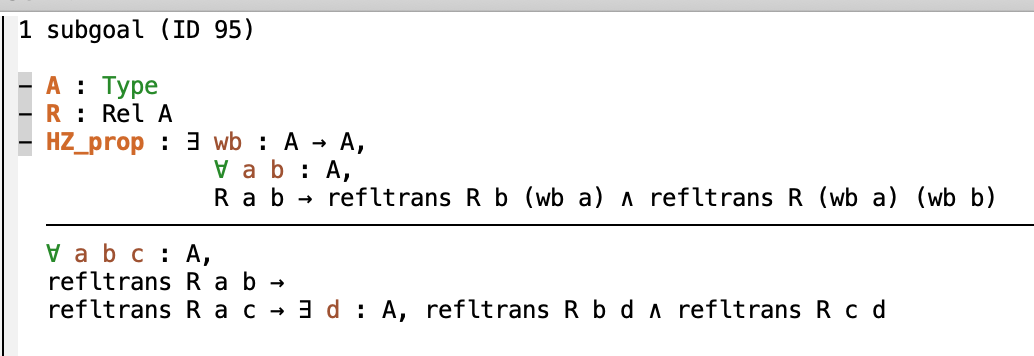
\includegraphics[scale=0.6]{fig3.png} \begin{coqdoccode}
\coqdocemptyline
\coqdocindent{1.00em}
\coqdoctac{intros} \coqdocvar{a} \coqdocvar{b} \coqdocvar{c} \coqdocvar{Hrefl1} \coqdocvar{Hrefl2}. \end{coqdoccode}
Let \coqdocvar{a}, \coqdocvar{b} and \coqdocvar{c} be elements of
     the set \coqdocvar{A}, \coqdocvar{Hrefl1} the hypothesis that $a \tto_R b$, and
     \coqdocvar{Hrefl2} the hypothesis that $a\tto_R c$.  \begin{coqdoccode}
\coqdocemptyline
\coqdocindent{1.00em}
\coqdoctac{destruct} \coqdocvar{HZ\_prop} \coqdockw{as} [\coqdocvar{g} \coqdocvar{HZ\_prop}]. \end{coqdoccode}
In addition, by the hypothesis
     \coqdocvar{HZ\_prop}, we know that there exists a mapping \coqdocvar{f} that is
     Z. Let's call \coqdocvar{g} this mapping, and we get following proof
     context:


      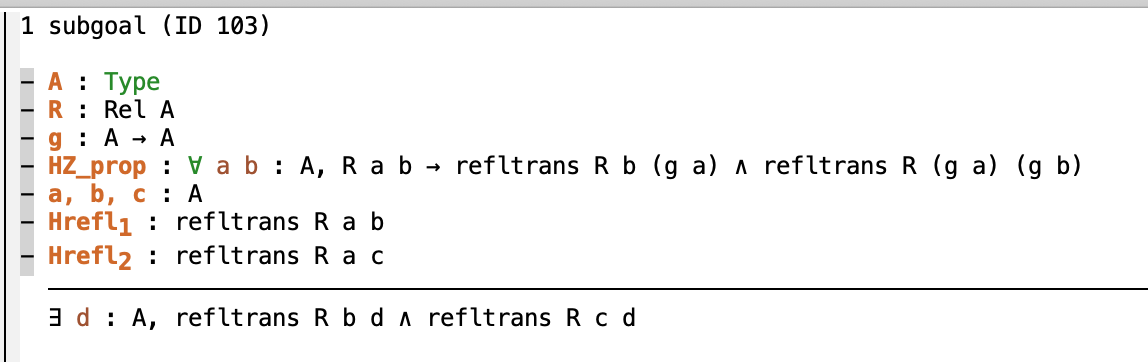
\includegraphics[scale=0.6]{fig4.png}


      Now we need to show that there exists an element \coqdocvar{d} such that
      both \coqdocvar{b} and \coqdocvar{c} \coqdocvar{R}-reduces to \coqdocvar{d}. The proof proceeds by
      nested induction, firstly on the length of the reduction from
      \coqdocvar{a} to \coqdocvar{b}, and then on the length of the reduction from \coqdocvar{a} to
      \coqdocvar{c}. \begin{coqdoccode}
\coqdocemptyline
\coqdocindent{1.00em}
\coqdoctac{generalize} \coqdoctac{dependent} \coqdocvar{c}. \end{coqdoccode}
Before the first induction,
      i.e. induction on \coqdocvar{Hrefl1}, the element \coqdocvar{c} needs to be
      generalized so that it can be afterwards instantiated with any
      reduct of \coqdocvar{a}. \begin{coqdoccode}
\coqdocemptyline
\coqdocindent{1.00em}
\coqdoctac{induction} \coqdocvar{Hrefl1}. \end{coqdoccode}
The induction on \coqdocvar{Hrefl1} corresponds to
       induction on the reflexive transitive closure of the relation
       \coqdocvar{R}, and since \coqdocvar{refltrans} has two rules, the goal split in two
       subgoals, one for each possible way of constructing $a \tto_R
       b$. \begin{coqdoccode}
\coqdocemptyline
\coqdocindent{1.00em}
- \coqdoctac{intros} \coqdocvar{c} \coqdocvar{Hrefl2}. \end{coqdoccode}
In the first case, $a = b$ since we are in
    the reflexive case. \begin{coqdoccode}
\coqdocemptyline
\coqdocindent{2.00em}
\coqdoctac{\ensuremath{\exists}} \coqdocvar{c}; \coqdoctac{split}. \end{coqdoccode}
Therefore, there is no divergence and this case is
      proved by taking \coqdocvar{c} as \coqdocvar{d}. \begin{coqdoccode}
\coqdocemptyline
\coqdocindent{2.00em}
+ \coqdoctac{assumption}. \end{coqdoccode}
The goal is then the conjunction $a\tto_R c
        \land c \tto_R c$ whose first component is exactly the
        hypothesis \coqdocvar{Hrefl2} and, \begin{coqdoccode}
\coqdocemptyline
\coqdocindent{2.00em}
+ \coqdoctac{apply} \coqref{ZtoConfl.refl}{\coqdocconstructor{refl}}. \end{coqdoccode}
$c \tto_R c$ corresponds to an application of
        the \coqdocvar{refl} axiom.


        The interesting case is given by the inductive case, i.e. by
        the rule (\coqdocvar{rtrans}), where the reduction from \coqdocvar{a} to \coqdocvar{b} is
        done in at least one step. Therefore, there exists an element
        $a'$ such that the following diagram holds.


         \[\xymatrix{ & & a \ar@{->}[dl] \ar@{->>}[dr] & \\ & a'
        \ar@{->>}[dl] & & c \ar@{.>>}[ddll] \\ b \ar@{.>>}[dr] & & &
        \\ & d & & }\] 


        

        The induction hypothesis states that every divergence from
        $a'$, that reduces to $b$ from one side, converges: \coqdocvar{IHHrefl1}
        : $\forall c_0 : A, a'\tto_R c_0 \to (\exists d : A, b\tto_R d
        \land c_0\tto_R d$). The idea is to apply induction on the
        hypothesis \coqdocvar{Hrefl2}, but the current proof context has the
        hypothesis \coqdocvar{H}: $a\to_R a'$, which will generate, in the
        induction hypothesis, the condition that $a'\to_R c$, and this
        is not true in general. In order to circumvent this problem,
        we need to remove this hypothesis, but the information that
        $a\to_R b$ is essential and cannot be simply removed. At this
        point, we use the Z property as shown below. \begin{coqdoccode}
\coqdocemptyline
\coqdocindent{1.00em}
- \coqdoctac{intros} \coqdocvar{c0} \coqdocvar{Hrefl2}. \end{coqdoccode}
Let $c_0$ be a reduct of $b$, and \coqdocvar{Hrefl2}
    the fact that $a \tto_R c_0$. So the reduction $a\tto_R c$ in the
    above diagrams is now $a\tto_R c_0$ due to a renaming of variables
    automatically done by the Coq system. Before applying induction to
    \coqdocvar{Hrefl2}: $a \tto_R c_0$, we will be replace the hypothesis \coqdocvar{H} by
    two other properties that are proved from the Z property: $b\tto_R
    (g\ a)$ and $a\tto_R (g\ a)$. \begin{coqdoccode}
\coqdocemptyline
\coqdocindent{2.00em}
\coqdoctac{assert} (\coqdocvar{H1}: \coqref{ZtoConfl.refltrans}{\coqdocinductive{refltrans}} \coqdocvar{R} \coqdocvar{b} (\coqdocvar{g} \coqdocvar{a})).\coqdoceol
\coqdocindent{2.00em}
\{ \coqdoctac{apply} \coqdocvar{HZ\_prop}; \coqdoctac{assumption}. \} \end{coqdoccode}
We call \coqdocvar{H1} the reduction
    $b\tto_R (g\ a)$ that is directly obtained from the Z property.
    \begin{coqdoccode}
\coqdocnoindent
\coqdoceol
\coqdocindent{2.00em}
\coqdoctac{assert} (\coqdocvar{H2}: \coqref{ZtoConfl.refltrans}{\coqdocinductive{refltrans}} \coqdocvar{R} \coqdocvar{a} (\coqdocvar{g} \coqdocvar{a})).\coqdoceol
\coqdocindent{2.00em}
\{ \coqdoctac{apply} \coqref{ZtoConfl.rtrans}{\coqdocconstructor{rtrans}} \coqdockw{with} \coqdocvar{b}; \coqdoctac{assumption}. \} \end{coqdoccode}
Call \coqdocvar{H2} the reduction
        $a\tto_R (g\ a)$, and prove it using the transitivity of
        $\tto_R$, since $a \to_R b$ and $b \tto_R (g\ a)$.


        Diagrammatically, we change from the situation on the left to
        the one on the right:


        \begin{tabular}{c@{\hskip 0.5cm}c} $\xymatrix{ & & a
        \ar@{->>}[ddrr]_R \ar@{->}[dl]^R & & \\ & a' \ar@{->>}[dl]^R &
        & & \\ b \ar@{.>>}[ddrr]_R & & & & c \ar@{.>>}[ddll]^R \\ & &
        & & \\ & & d & & }$ & $\xymatrix{ & & a \ar@{->>}[ddrr]_R
        \ar@{->>}[dd]_R & & \\ & a' \ar@{->>}[dl]^R \ar@{->>}[dr]_R &
        & & \\ b \ar@{.>>}[ddrr]_R & & (g \; a) & & c
        \ar@{.>>}[ddll]^R \\ & & & & \\ & & d & & }$ \end{tabular} \begin{coqdoccode}
\coqdocnoindent
\coqdoceol
\coqdocindent{2.00em}
\coqdoctac{clear} \coqdocvar{H}; \coqdoctac{generalize} \coqdoctac{dependent} \coqdocvar{b}. \end{coqdoccode}
At this point we can remove
      the hypothesis \coqdocvar{H} from the context, and generalize \coqdocvar{b}. \begin{coqdoccode}
\coqdocemptyline
\coqdocindent{2.00em}
\coqdoctac{induction} \coqdocvar{Hrefl2}. \end{coqdoccode}
Now we are ready to start the induction on
    the reduction $a\tto_R c_0$, and we have two subgoals. \begin{coqdoccode}
\coqdocemptyline
\coqdocindent{2.00em}
+ \coqdoctac{intros} \coqdocvar{b} \coqdocvar{Hrefl1} \coqdocvar{IHHrefl1} \coqdocvar{H1}. \end{coqdoccode}
The first subgoal corresponds
        to the reflexive case, that is closed by the induction
        hypothesis \coqdocvar{IHHrefl1}:


        \[\xymatrix{ & & a \ar@{->>}[dd]^{H2} & & \\ & b
        \ar@{->>}[dl]_{Hrefl1} \ar@{->>}[dr]^{H1} & & & \\ c
        \ar@{.>>}[dr] & IHHrefl1 & (g \; a) \ar@{.>>}[dl] & & \\ & d &
        &&}\] \begin{coqdoccode}
\coqdocemptyline
\coqdocindent{3.00em}
\coqdoctac{assert} (\coqdocvar{IHHrefl1\_ga} := \coqdocvar{IHHrefl1} (\coqdocvar{g} \coqdocvar{a})); \coqdoctac{apply} \coqdocvar{IHHrefl1\_ga} \coqdoctac{in} \coqdocvar{H1}. \end{coqdoccode}
      In order to apply \coqdocvar{IHHrefl1}, we instantiate $c_0$ with $(g\
      a)$. \begin{coqdoccode}
\coqdocemptyline
\coqdocindent{3.00em}
\coqdoctac{destruct} \coqdocvar{H1}. \end{coqdoccode}
Therefore, there exists an element, say $x$,
      such that both $c\tto_R x$ and $(g\ a) \tto_R x$. \begin{coqdoccode}
\coqdocemptyline
\coqdocindent{3.00em}
\coqdoctac{\ensuremath{\exists}} \coqdocvar{x}; \coqdoctac{split}. \end{coqdoccode}
We then take $x$ to show that $c\tto_R x$ and $a
      \tto_R x$. \begin{coqdoccode}
\coqdocemptyline
\coqdocindent{3.00em}
\ensuremath{\times} \coqdoctac{apply} \coqdocvar{H}. \end{coqdoccode}
Note that $c\tto_R x$ is already an hypothesis,
        and we are done. \begin{coqdoccode}
\coqdocemptyline
\coqdocindent{3.00em}
\ensuremath{\times} \coqdoctac{apply} \coqref{ZtoConfl.refltrans composition}{\coqdoclemma{refltrans\_composition}} \coqdockw{with} (\coqdocvar{g} \coqdocvar{a}); [\coqdoctac{assumption} \ensuremath{|} \coqdoctac{apply} \coqdocvar{H}]. \end{coqdoccode}
      The proof of $a \tto_R x$ is done by the transitivity of
      $\tto_R$ taking $(g\ a)$ as the intermediary step. \begin{coqdoccode}
\coqdocemptyline
\coqdocindent{2.00em}
+ \coqdoctac{intros} \coqdocvar{b0} \coqdocvar{Hrefl1} \coqdocvar{IHHrefl1} \coqdocvar{H'}. \end{coqdoccode}
The second subgoal corresponds
        to the case in which $a\tto_R c_0$ is generated by the rule
        $(rtrans)$. Therefore, there exists a term $b$ such that
        $a\to_R b$ and $b \tto_R c_0$. The corresponding proof context
        after introducing the universally quantified variable \coqdocvar{b0},
        the hypothesis \coqdocvar{Hrefl1} and the induction hypothesis
        \coqdocvar{IHHrefl1} generated by the first outer induction and the fact
        that $b0 \tto_R (g\ a)$ is given by:


        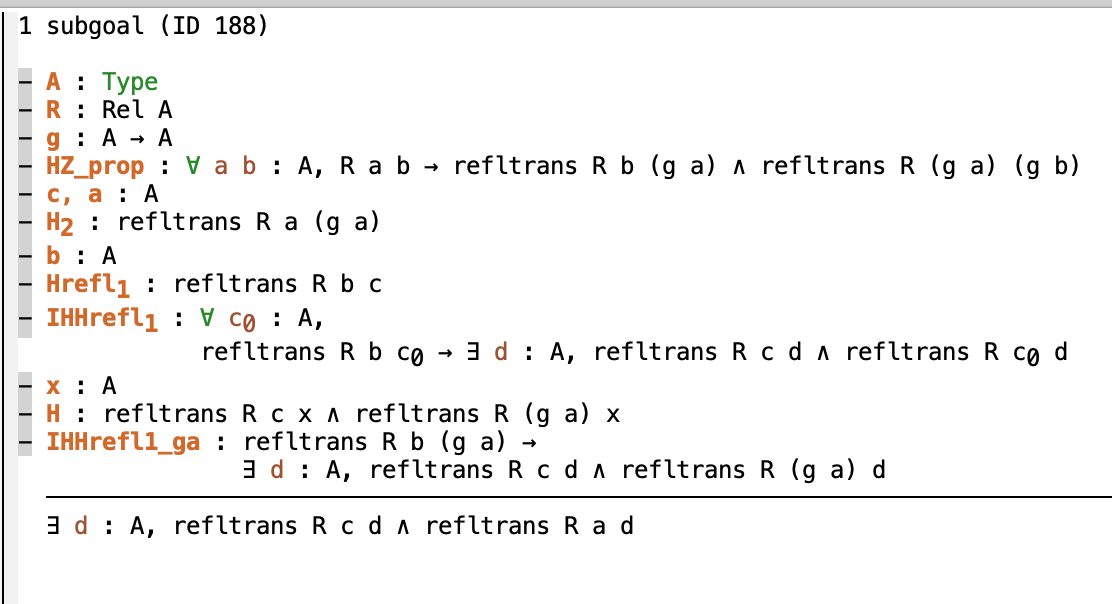
\includegraphics[scale=0.6]{fig7.png} \begin{coqdoccode}
\coqdocemptyline
\coqdocindent{3.00em}
\coqdoctac{apply} \coqdocvar{IHHrefl2} \coqdockw{with} \coqdocvar{b0}. \end{coqdoccode}
The second goal, i.e. the inductive
        case can be proved by the second induction hypothesis
        \coqdocvar{IHHrefl2}, and each of the 4 conditions generated by this
        hypothesis is solved as follows: \begin{coqdoccode}
\coqdocemptyline
\coqdocindent{3.00em}
\ensuremath{\times} \coqdoctac{apply} \coqref{ZtoConfl.refltrans composition}{\coqdoclemma{refltrans\_composition}} \coqdockw{with} (\coqdocvar{g} \coqdocvar{a}); \coqdoctac{apply} \coqdocvar{HZ\_prop}; \coqdoctac{assumption}. \end{coqdoccode}
      1. $b \tto_R (g\ b)$: This is proved by the transitivity of the
      reflexive transitive closure of \coqdocvar{R} using the
      hypothesis (H: $a\to_R b$) and \coqdocvar{HZ\_prop}: $\forall a\
      b: a \to_R b \to (b \tto_R (g\ a) \land (g\ a) \tto_R (g\ b))$. \begin{coqdoccode}
\coqdocemptyline
\coqdocindent{3.00em}
\ensuremath{\times} \coqdoctac{assumption}. \end{coqdoccode}
2. $b0 \tto_R c$: This is exactly the
          hypothesis \coqdocvar{Hrefl1}. \begin{coqdoccode}
\coqdocemptyline
\coqdocindent{3.00em}
\ensuremath{\times} \coqdoctac{assumption}. \end{coqdoccode}
3. $\forall c0: b0 \tto_R c0 \to (\exists d:
            c \tto_R d \land c0 \tto_R d)$: This is exactly the
            induction hypothesis \coqdocvar{IHHrefl1}. \begin{coqdoccode}
\coqdocemptyline
\coqdocindent{3.00em}
\ensuremath{\times} \coqdoctac{apply} \coqref{ZtoConfl.refltrans composition}{\coqdoclemma{refltrans\_composition}} \coqdockw{with} (\coqdocvar{g} \coqdocvar{a}); [ \coqdoctac{assumption} \ensuremath{|} \coqdoctac{apply} \coqdocvar{HZ\_prop}; \coqdoctac{assumption}]. \end{coqdoccode}
      4. $b0 \tto_R (g\ b)$: This is proved by the transitivity of
      the reflexive transitive closure of \coqdocvar{R} using the
      hypothesis (\coqdocvar{H'}: $b0 \tto_R (g\ a)$ and the fact that
      $(g\ a) \tto_R (g\ b)$ that is obtained from the fact that
      \coqdocvar{R} satisfies the Z property (hypothesis
      \coqdocvar{HZ\_prop}). \begin{coqdoccode}
\coqdocemptyline
\coqdocnoindent
\coqdockw{Qed}.\coqdoceol
\coqdocemptyline
\end{coqdoccode}
An alternative proof that Z implies confluence is possible via the
    notion of semiconfluence, which is equivalent to confluence, as
    done in \cite{zproperty}. Our proof is also constructive, but we
    will not explain it here due to lack of space, but as the
    interested reader can visit the Coq file in our GitHub
    repository. \begin{coqdoccode}
\coqdocemptyline
\coqdocnoindent
\coqdockw{Lemma} \coqdef{ZtoConfl.red to f}{red\_to\_f}{\coqdoclemma{red\_to\_f}} \{\coqdocvar{A}: \coqdockw{Type}\}: \coqdockw{\ensuremath{\forall}} (\coqdocvar{R}: \coqref{ZtoConfl.Rel}{\coqdocdefinition{Rel}} \coqdocvariable{A}) (\coqdocvar{f}: \coqdocvariable{A} \coqexternalref{::type scope:x '->' x}{http://coq.inria.fr/distrib/V8.11.0/stdlib//Coq.Init.Logic}{\coqdocnotation{\ensuremath{\rightarrow}}} \coqdocvariable{A}), \coqref{ZtoConfl.f is Z}{\coqdocdefinition{f\_is\_Z}} \coqdocvariable{R} \coqdocvariable{f} \coqexternalref{::type scope:x '->' x}{http://coq.inria.fr/distrib/V8.11.0/stdlib//Coq.Init.Logic}{\coqdocnotation{\ensuremath{\rightarrow}}} \coqexternalref{::type scope:x '->' x}{http://coq.inria.fr/distrib/V8.11.0/stdlib//Coq.Init.Logic}{\coqdocnotation{(}}\coqdockw{\ensuremath{\forall}} \coqdocvar{a} \coqdocvar{b}: \coqdocvariable{A}, \coqref{ZtoConfl.refltrans}{\coqdocinductive{refltrans}} \coqdocvariable{R} \coqdocvariable{a} \coqdocvariable{b} \coqexternalref{::type scope:x '->' x}{http://coq.inria.fr/distrib/V8.11.0/stdlib//Coq.Init.Logic}{\coqdocnotation{\ensuremath{\rightarrow}}} \coqref{ZtoConfl.refltrans}{\coqdocinductive{refltrans}} \coqdocvariable{R} (\coqdocvariable{f} \coqdocvariable{a}) (\coqdocvariable{f} \coqdocvariable{b})\coqexternalref{::type scope:x '->' x}{http://coq.inria.fr/distrib/V8.11.0/stdlib//Coq.Init.Logic}{\coqdocnotation{)}}. \coqdockw{Proof}. \coqdoctac{intros} \coqdocvar{R} \coqdocvar{f} \coqdocvar{H} \coqdocvar{a} \coqdocvar{b} \coqdocvar{Hred}. \coqdoctac{unfold} \coqref{ZtoConfl.f is Z}{\coqdocdefinition{f\_is\_Z}} \coqdoctac{in} \coqdocvar{H}. \coqdoctac{induction} \coqdocvar{Hred}. - \coqdoctac{apply} \coqref{ZtoConfl.refl}{\coqdocconstructor{refl}}. - \coqdoctac{apply} \coqref{ZtoConfl.refltrans composition}{\coqdoclemma{refltrans\_composition}} \coqdockw{with} (\coqdocvar{f} \coqdocvar{b}). + \coqdoctac{apply} \coqdocvar{H}; \coqdoctac{assumption}. + \coqdoctac{assumption}. \coqdockw{Qed}.\coqdoceol
\coqdocemptyline
\coqdocnoindent
\coqdockw{Definition} \coqdef{ZtoConfl.SemiConfl}{SemiConfl}{\coqdocdefinition{SemiConfl}} \{\coqdocvar{A}:\coqdockw{Type}\} (\coqdocvar{R}: \coqref{ZtoConfl.Rel}{\coqdocdefinition{Rel}} \coqdocvariable{A}) := \coqdockw{\ensuremath{\forall}} \coqdocvar{a} \coqdocvar{b} \coqdocvar{c}, \coqdocvariable{R} \coqdocvariable{a} \coqdocvariable{b} \coqexternalref{::type scope:x '->' x}{http://coq.inria.fr/distrib/V8.11.0/stdlib//Coq.Init.Logic}{\coqdocnotation{\ensuremath{\rightarrow}}} (\coqref{ZtoConfl.refltrans}{\coqdocinductive{refltrans}} \coqdocvariable{R}) \coqdocvariable{a} \coqdocvariable{c} \coqexternalref{::type scope:x '->' x}{http://coq.inria.fr/distrib/V8.11.0/stdlib//Coq.Init.Logic}{\coqdocnotation{\ensuremath{\rightarrow}}} \coqexternalref{::type scope:x '->' x}{http://coq.inria.fr/distrib/V8.11.0/stdlib//Coq.Init.Logic}{\coqdocnotation{(}}\coqexternalref{::type scope:'exists' x '..' x ',' x}{http://coq.inria.fr/distrib/V8.11.0/stdlib//Coq.Init.Logic}{\coqdocnotation{\ensuremath{\exists}}} \coqdocvar{d}\coqexternalref{::type scope:'exists' x '..' x ',' x}{http://coq.inria.fr/distrib/V8.11.0/stdlib//Coq.Init.Logic}{\coqdocnotation{,}} (\coqref{ZtoConfl.refltrans}{\coqdocinductive{refltrans}} \coqdocvariable{R}) \coqdocvariable{b} \coqdocvariable{d} \coqexternalref{::type scope:x '/x5C' x}{http://coq.inria.fr/distrib/V8.11.0/stdlib//Coq.Init.Logic}{\coqdocnotation{\ensuremath{\land}}} (\coqref{ZtoConfl.refltrans}{\coqdocinductive{refltrans}} \coqdocvariable{R}) \coqdocvariable{c} \coqdocvariable{d}\coqexternalref{::type scope:x '->' x}{http://coq.inria.fr/distrib/V8.11.0/stdlib//Coq.Init.Logic}{\coqdocnotation{)}}.\coqdoceol
\coqdocemptyline
\coqdocnoindent
\coqdockw{Theorem} \coqdef{ZtoConfl.Z prop implies SemiConfl}{Z\_prop\_implies\_SemiConfl}{\coqdoclemma{Z\_prop\_implies\_SemiConfl}} \{\coqdocvar{A}:\coqdockw{Type}\}: \coqdockw{\ensuremath{\forall}} \coqdocvar{R}: \coqref{ZtoConfl.Rel}{\coqdocdefinition{Rel}} \coqdocvariable{A}, \coqref{ZtoConfl.Z prop}{\coqdocdefinition{Z\_prop}} \coqdocvariable{R} \coqexternalref{::type scope:x '->' x}{http://coq.inria.fr/distrib/V8.11.0/stdlib//Coq.Init.Logic}{\coqdocnotation{\ensuremath{\rightarrow}}} \coqref{ZtoConfl.SemiConfl}{\coqdocdefinition{SemiConfl}} \coqdocvariable{R}.  \coqdockw{Proof}. \coqdoctac{intros} \coqdocvar{R} \coqdocvar{HZ\_prop}. \coqdoctac{unfold} \coqref{ZtoConfl.Z prop}{\coqdocdefinition{Z\_prop}} \coqdoctac{in} \coqdocvar{HZ\_prop}. \coqdoctac{unfold} \coqref{ZtoConfl.SemiConfl}{\coqdocdefinition{SemiConfl}}. \coqdoctac{destruct} \coqdocvar{HZ\_prop}. \coqdoctac{intros} \coqdocvar{a} \coqdocvar{b} \coqdocvar{c} \coqdocvar{Hrefl} \coqdocvar{Hrefl'}. \coqdoctac{assert} (\coqdocvar{Haxa}: \coqref{ZtoConfl.refltrans}{\coqdocinductive{refltrans}} \coqdocvar{R} \coqdocvar{a} (\coqdocvar{x} \coqdocvar{a})). \{ \coqdoctac{apply} \coqref{ZtoConfl.rtrans}{\coqdocconstructor{rtrans}} \coqdockw{with} \coqdocvar{b}. - \coqdoctac{assumption}. - \coqdoctac{apply} \coqdocvar{H}. \coqdoctac{assumption}. \} \coqdoctac{apply} \coqdocvar{H} \coqdoctac{in} \coqdocvar{Hrefl}. \coqdoctac{destruct} \coqdocvar{Hrefl}. \coqdoctac{clear} \coqdocvar{H1}. \coqdoctac{generalize} \coqdoctac{dependent} \coqdocvar{b}. \coqdoctac{induction} \coqdocvar{Hrefl'}. - \coqdoctac{intros}. \coqdoctac{\ensuremath{\exists}} (\coqdocvar{x} \coqdocvar{a}). \coqdoctac{split}; \coqdoctac{assumption}. - \coqdoctac{intros}. \coqdoctac{destruct} \coqdocvar{IHHrefl'} \coqdockw{with} \coqdocvar{b0}. + \coqdoctac{apply} \coqref{ZtoConfl.refltrans composition}{\coqdoclemma{refltrans\_composition}} \coqdockw{with} (\coqdocvar{x} \coqdocvar{a}); \coqdoctac{apply} \coqdocvar{H}; \coqdoctac{assumption}. + \coqdoctac{apply} \coqref{ZtoConfl.refltrans composition}{\coqdoclemma{refltrans\_composition}} \coqdockw{with} (\coqdocvar{x} \coqdocvar{b}). \ensuremath{\times} \coqdoctac{apply} \coqref{ZtoConfl.refltrans composition}{\coqdoclemma{refltrans\_composition}} \coqdockw{with} (\coqdocvar{x} \coqdocvar{a}). ** \coqdoctac{assumption}. ** \coqdoctac{apply} \coqdocvar{H}. \coqdoctac{assumption}. \ensuremath{\times} \coqdoctac{apply} \coqref{ZtoConfl.refl}{\coqdocconstructor{refl}}. + \coqdoctac{\ensuremath{\exists}} \coqdocvar{x0}. \coqdoctac{assumption}. \coqdockw{Qed}. \coqdocemptyline
\coqdocnoindent
\coqdockw{Theorem} \coqdef{ZtoConfl.Semi equiv Confl}{Semi\_equiv\_Confl}{\coqdoclemma{Semi\_equiv\_Confl}} \{\coqdocvar{A}: \coqdockw{Type}\}: \coqdockw{\ensuremath{\forall}} \coqdocvar{R}: \coqref{ZtoConfl.Rel}{\coqdocdefinition{Rel}} \coqdocvariable{A}, \coqref{ZtoConfl.Confl}{\coqdocdefinition{Confl}} \coqdocvariable{R} \coqexternalref{::type scope:x '<->' x}{http://coq.inria.fr/distrib/V8.11.0/stdlib//Coq.Init.Logic}{\coqdocnotation{\ensuremath{\leftrightarrow}}} \coqref{ZtoConfl.SemiConfl}{\coqdocdefinition{SemiConfl}} \coqdocvariable{R}.  \coqdockw{Proof}. \coqdoctac{unfold} \coqref{ZtoConfl.Confl}{\coqdocdefinition{Confl}}. \coqdoctac{unfold} \coqref{ZtoConfl.SemiConfl}{\coqdocdefinition{SemiConfl}}. \coqdoctac{intro} \coqdocvar{R}. \coqdoctac{split}. - \coqdoctac{intros}. \coqdoctac{apply} \coqdocvar{H} \coqdockw{with} \coqdocvar{a}. + \coqdoctac{apply} \coqref{ZtoConfl.rtrans}{\coqdocconstructor{rtrans}} \coqdockw{with} \coqdocvar{b}. \ensuremath{\times} \coqdoctac{assumption}. \ensuremath{\times} \coqdoctac{apply} \coqref{ZtoConfl.refl}{\coqdocconstructor{refl}}. + \coqdoctac{assumption}. - \coqdoctac{intros}. \coqdoctac{generalize} \coqdoctac{dependent} \coqdocvar{c}. \coqdoctac{induction} \coqdocvar{H0}. + \coqdoctac{intros}. \coqdoctac{\ensuremath{\exists}} \coqdocvar{c}. \coqdoctac{split}. \ensuremath{\times} \coqdoctac{assumption}. \ensuremath{\times} \coqdoctac{apply} \coqref{ZtoConfl.refl}{\coqdocconstructor{refl}}. + \coqdoctac{intros}. \coqdoctac{specialize} (\coqdocvar{H} \coqdocvar{a}). \coqdoctac{specialize} (\coqdocvar{H} \coqdocvar{b}). \coqdoctac{specialize} (\coqdocvar{H} \coqdocvar{c0}). \coqdoctac{apply} \coqdocvar{H} \coqdoctac{in} \coqdocvar{H0}. \ensuremath{\times} \coqdoctac{destruct} \coqdocvar{H0}. \coqdoctac{destruct} \coqdocvar{H0}. \coqdoctac{apply} \coqdocvar{IHrefltrans} \coqdoctac{in} \coqdocvar{H0}. \coqdoctac{destruct} \coqdocvar{H0}. \coqdoctac{destruct} \coqdocvar{H0}. \coqdoctac{\ensuremath{\exists}} \coqdocvar{x0}. \coqdoctac{split}. ** \coqdoctac{assumption}. ** \coqdoctac{apply} \coqref{ZtoConfl.refltrans composition}{\coqdoclemma{refltrans\_composition}} \coqdockw{with} \coqdocvar{x}; \coqdoctac{assumption}. \ensuremath{\times} \coqdoctac{assumption}. \coqdockw{Qed}. \coqdocemptyline
\end{coqdoccode}
\section{An extension of the Z property: Compositional Z}




    In this section we present a formalization of an extension of the
    Z property with compositional functions, known as \textit{Compositional
    Z}, as presented in \cite{Nakazawa-Fujita2016}. The
    compositional Z is an interesting property because it allows a
    kind of modular approach to the Z property in such a way that the
    reduction relation can be split into two parts. More precisely,
    given an ARS $(A,\to)$, one must be able to decompose the relation
    $\to$ into two parts, say $\to_1$ and $\to_2$ such that $\to =
    \to_1\cup \to_2$. The disjoint union can be inductively defined in
    Coq as follows: \begin{coqdoccode}
\coqdocemptyline
\coqdocnoindent
\coqdockw{Inductive} \coqdef{ZtoConfl.union}{union}{\coqdocinductive{union}} \{\coqdocvar{A}\} (\coqdocvar{red1} \coqdocvar{red2}: \coqref{ZtoConfl.Rel}{\coqdocdefinition{Rel}} \coqdocvariable{A}) : \coqref{ZtoConfl.Rel}{\coqdocdefinition{Rel}} \coqdocvar{A} := \ensuremath{|} \coqdef{ZtoConfl.union left}{union\_left}{\coqdocconstructor{union\_left}}: \coqdockw{\ensuremath{\forall}} \coqdocvar{a} \coqdocvar{b}, \coqdocvariable{red1} \coqdocvariable{a} \coqdocvariable{b} \coqexternalref{::type scope:x '->' x}{http://coq.inria.fr/distrib/V8.11.0/stdlib//Coq.Init.Logic}{\coqdocnotation{\ensuremath{\rightarrow}}} \coqref{ZtoConfl.union}{\coqdocinductive{union}} \coqdocvariable{red1} \coqdocvariable{red2} \coqdocvariable{a} \coqdocvariable{b} \ensuremath{|} \coqdef{ZtoConfl.union right}{union\_right}{\coqdocconstructor{union\_right}}: \coqdockw{\ensuremath{\forall}} \coqdocvar{a} \coqdocvar{b}, \coqdocvariable{red2} \coqdocvariable{a} \coqdocvariable{b} \coqexternalref{::type scope:x '->' x}{http://coq.inria.fr/distrib/V8.11.0/stdlib//Coq.Init.Logic}{\coqdocnotation{\ensuremath{\rightarrow}}} \coqref{ZtoConfl.union}{\coqdocinductive{union}} \coqdocvariable{red1} \coqdocvariable{red2} \coqdocvariable{a} \coqdocvariable{b}.\coqdoceol
\coqdocemptyline
\coqdocnoindent
\coqdockw{Notation} \coqdef{ZtoConfl.:::x '! !' x}{"}{"}R1 !\_! R2" := (\coqref{ZtoConfl.union}{\coqdocinductive{union}} \coqdocvar{R1} \coqdocvar{R2}) (\coqdoctac{at} \coqdockw{level} 40).\coqdoceol
\coqdocemptyline
\end{coqdoccode}
This kind of decomposition can be done in several interesting
situations such as the $\lambda$-calculus with
$\beta\eta$-reduction\cite{Ba84}, extensions of the
$\lambda$-calculus with explicit substitutions\cite{accl91}, the
$\lambda\mu$-calculus\cite{Parigot92}, etc.  \begin{coqdoccode}
\coqdocemptyline
 \coqdockw{Lemma} \coqdef{ZtoConfl.union or}{union\_or}{\coqdoclemma{union\_or}} \{\coqdocvar{A}\}: \coqdockw{\ensuremath{\forall}} (\coqdocvar{r1} \coqdocvar{r2}: \coqref{ZtoConfl.Rel}{\coqdocdefinition{Rel}} \coqdocvariable{A}) (\coqdocvar{a} \coqdocvar{b}: \coqdocvariable{A}), (\coqdocvariable{r1} \coqref{ZtoConfl.:::x '! !' x}{\coqdocnotation{!}}\coqref{ZtoConfl.:::x '! !' x}{\coqdocnotation{\_}}\coqref{ZtoConfl.:::x '! !' x}{\coqdocnotation{!}} \coqdocvariable{r2}) \coqdocvariable{a} \coqdocvariable{b} \coqexternalref{::type scope:x '<->' x}{http://coq.inria.fr/distrib/V8.11.0/stdlib//Coq.Init.Logic}{\coqdocnotation{\ensuremath{\leftrightarrow}}} \coqexternalref{::type scope:x 'x5C/' x}{http://coq.inria.fr/distrib/V8.11.0/stdlib//Coq.Init.Logic}{\coqdocnotation{(}}\coqdocvariable{r1} \coqdocvariable{a} \coqdocvariable{b}\coqexternalref{::type scope:x 'x5C/' x}{http://coq.inria.fr/distrib/V8.11.0/stdlib//Coq.Init.Logic}{\coqdocnotation{)}} \coqexternalref{::type scope:x 'x5C/' x}{http://coq.inria.fr/distrib/V8.11.0/stdlib//Coq.Init.Logic}{\coqdocnotation{\ensuremath{\lor}}} \coqexternalref{::type scope:x 'x5C/' x}{http://coq.inria.fr/distrib/V8.11.0/stdlib//Coq.Init.Logic}{\coqdocnotation{(}}\coqdocvariable{r2} \coqdocvariable{a} \coqdocvariable{b}\coqexternalref{::type scope:x 'x5C/' x}{http://coq.inria.fr/distrib/V8.11.0/stdlib//Coq.Init.Logic}{\coqdocnotation{)}}. \coqdockw{Proof}. \coqdoctac{intros} \coqdocvar{r1} \coqdocvar{r2} \coqdocvar{a} \coqdocvar{b}; \coqdoctac{split}. - \coqdoctac{intro} \coqdocvar{Hunion}. \coqdoctac{inversion} \coqdocvar{Hunion}; \coqdoctac{subst}. + \coqdoctac{left}; \coqdoctac{assumption}. + \coqdoctac{right}; \coqdoctac{assumption}. - \coqdoctac{intro} \coqdocvar{Hunion}. \coqdoctac{inversion} \coqdocvar{Hunion}. + \coqdoctac{apply} \coqref{ZtoConfl.union left}{\coqdocconstructor{union\_left}}; \coqdoctac{assumption}. + \coqdoctac{apply} \coqref{ZtoConfl.union right}{\coqdocconstructor{union\_right}}; \coqdoctac{assumption}. \coqdockw{Qed}. \coqdocemptyline
\end{coqdoccode}
The compositional Z is defined in terms of a weaker property:


    \begin{definition} Let $(A,\to)$ be an ARS and $\to_x$ another
     relation on $A$. A mapping $f$ satisfies the {\it weak Z
     property} for $\to$ by $\to_x$ if $a\to b$ implies $b \tto_x
     f(a)$ and $f(a) \tto_x f(b)$. Therefore, a mapping $f$ satisfies
     the Z property for $\to$, if it satisfies the weak Z property by
     itself.  \end{definition}


    When $f$ satisfies the weak Z property, we also say that $f$ is
    weakly Z, and the corresponding definition in Coq is given as
    follows: \begin{coqdoccode}
\coqdocemptyline
\coqdocnoindent
\coqdockw{Definition} \coqdef{ZtoConfl.f is weak Z}{f\_is\_weak\_Z}{\coqdocdefinition{f\_is\_weak\_Z}} \{\coqdocvar{A}\} (\coqdocvar{R} \coqdocvar{R'}: \coqref{ZtoConfl.Rel}{\coqdocdefinition{Rel}} \coqdocvariable{A}) (\coqdocvar{f}: \coqdocvariable{A} \coqexternalref{::type scope:x '->' x}{http://coq.inria.fr/distrib/V8.11.0/stdlib//Coq.Init.Logic}{\coqdocnotation{\ensuremath{\rightarrow}}} \coqdocvariable{A}) := \coqdockw{\ensuremath{\forall}} \coqdocvar{a} \coqdocvar{b}, \coqdocvariable{R} \coqdocvariable{a} \coqdocvariable{b} \coqexternalref{::type scope:x '->' x}{http://coq.inria.fr/distrib/V8.11.0/stdlib//Coq.Init.Logic}{\coqdocnotation{\ensuremath{\rightarrow}}} \coqexternalref{::type scope:x '->' x}{http://coq.inria.fr/distrib/V8.11.0/stdlib//Coq.Init.Logic}{\coqdocnotation{(}}(\coqref{ZtoConfl.refltrans}{\coqdocinductive{refltrans}} \coqdocvariable{R'}) \coqdocvariable{b} (\coqdocvariable{f} \coqdocvariable{a}) \coqexternalref{::type scope:x '/x5C' x}{http://coq.inria.fr/distrib/V8.11.0/stdlib//Coq.Init.Logic}{\coqdocnotation{\ensuremath{\land}}} (\coqref{ZtoConfl.refltrans}{\coqdocinductive{refltrans}} \coqdocvariable{R'}) (\coqdocvariable{f} \coqdocvariable{a}) (\coqdocvariable{f} \coqdocvariable{b})\coqexternalref{::type scope:x '->' x}{http://coq.inria.fr/distrib/V8.11.0/stdlib//Coq.Init.Logic}{\coqdocnotation{)}}.\coqdoceol
\coqdocemptyline
\end{coqdoccode}
The compositional Z is an extension of the Z property for compositional functions, where composition is defined as usual: \begin{coqdoccode}
\coqdocemptyline
\coqdocnoindent
\coqdockw{Definition} \coqdef{ZtoConfl.comp}{comp}{\coqdocdefinition{comp}} \{\coqdocvar{A}\} (\coqdocvar{f1} \coqdocvar{f2}: \coqdocvariable{A} \coqexternalref{::type scope:x '->' x}{http://coq.inria.fr/distrib/V8.11.0/stdlib//Coq.Init.Logic}{\coqdocnotation{\ensuremath{\rightarrow}}} \coqdocvariable{A}) := \coqdockw{fun} \coqdocvar{x}:\coqdocvariable{A} \ensuremath{\Rightarrow} \coqdocvariable{f1} (\coqdocvariable{f2} \coqdocvariable{x}). \coqdockw{Notation} \coqdef{ZtoConfl.:::x 'x23' x}{"}{"}f1 \# f2" := (\coqref{ZtoConfl.comp}{\coqdocdefinition{comp}} \coqdocvar{f1} \coqdocvar{f2}) (\coqdoctac{at} \coqdockw{level} 40).\coqdoceol
\coqdocemptyline
\end{coqdoccode}
We are now ready to present the definition of the compositional Z:


    \begin{theorem}\cite{Nakazawa-Fujita2016}\label{thm:zcomp} Let $(A,\to)$ be an ARS such that $\to = \to_1 \cup \to_2$. If there exists mappings $f_1,f_2: A \to A$ such that \begin{enumerate} \item $f_1$ is Z for $\to_1$ \item $a \to_1 b$ implies $f_2(a) \tto f_2(b)$ \item $a \tto f_2(a)$ holds for any $a\in Im(f_1)$ \item $f_2 \circ f_1$ is weakly Z for $\to_2$ by $\to$ \end{enumerate} then $f_2 \circ f_1$ is Z for $(A,\to)$, and hence $(A,\to)$ is confluent.  \end{theorem}


    We define the predicate \coqdocvar{Z\_comp} that corresponds to the hypothesis of Theorem \ref{thm:zcomp}, where $\to_1$ (resp. $\to_2$) is written as \coqdocvar{R1} (resp. \coqdocvar{R2}): \begin{coqdoccode}
\coqdocemptyline
\coqdocnoindent
\coqdockw{Definition} \coqdef{ZtoConfl.Z comp}{Z\_comp}{\coqdocdefinition{Z\_comp}} \{\coqdocvar{A}:\coqdockw{Type}\} (\coqdocvar{R} :\coqref{ZtoConfl.Rel}{\coqdocdefinition{Rel}} \coqdocvariable{A}) := \coqexternalref{::type scope:'exists' x '..' x ',' x}{http://coq.inria.fr/distrib/V8.11.0/stdlib//Coq.Init.Logic}{\coqdocnotation{\ensuremath{\exists}}} \coqexternalref{::type scope:'exists' x '..' x ',' x}{http://coq.inria.fr/distrib/V8.11.0/stdlib//Coq.Init.Logic}{\coqdocnotation{(}}\coqdocvar{R1} \coqdocvar{R2}: \coqref{ZtoConfl.Rel}{\coqdocdefinition{Rel}} \coqdocvariable{A}) (\coqdocvar{f1} \coqdocvar{f2}: \coqdocvariable{A} \coqexternalref{::type scope:x '->' x}{http://coq.inria.fr/distrib/V8.11.0/stdlib//Coq.Init.Logic}{\coqdocnotation{\ensuremath{\rightarrow}}} \coqdocvariable{A}\coqexternalref{::type scope:'exists' x '..' x ',' x}{http://coq.inria.fr/distrib/V8.11.0/stdlib//Coq.Init.Logic}{\coqdocnotation{),}} \coqdocvariable{R} \coqexternalref{::type scope:x '=' x}{http://coq.inria.fr/distrib/V8.11.0/stdlib//Coq.Init.Logic}{\coqdocnotation{=}} \coqexternalref{::type scope:x '=' x}{http://coq.inria.fr/distrib/V8.11.0/stdlib//Coq.Init.Logic}{\coqdocnotation{(}}\coqdocvariable{R1} \coqref{ZtoConfl.:::x '! !' x}{\coqdocnotation{!}}\coqref{ZtoConfl.:::x '! !' x}{\coqdocnotation{\_}}\coqref{ZtoConfl.:::x '! !' x}{\coqdocnotation{!}} \coqdocvariable{R2}\coqexternalref{::type scope:x '=' x}{http://coq.inria.fr/distrib/V8.11.0/stdlib//Coq.Init.Logic}{\coqdocnotation{)}} \coqexternalref{::type scope:x '/x5C' x}{http://coq.inria.fr/distrib/V8.11.0/stdlib//Coq.Init.Logic}{\coqdocnotation{\ensuremath{\land}}} \coqref{ZtoConfl.f is Z}{\coqdocdefinition{f\_is\_Z}} \coqdocvariable{R1} \coqdocvariable{f1} \coqexternalref{::type scope:x '/x5C' x}{http://coq.inria.fr/distrib/V8.11.0/stdlib//Coq.Init.Logic}{\coqdocnotation{\ensuremath{\land}}} \coqexternalref{::type scope:x '/x5C' x}{http://coq.inria.fr/distrib/V8.11.0/stdlib//Coq.Init.Logic}{\coqdocnotation{(}}\coqdockw{\ensuremath{\forall}} \coqdocvar{a} \coqdocvar{b}, \coqdocvariable{R1} \coqdocvariable{a} \coqdocvariable{b} \coqexternalref{::type scope:x '->' x}{http://coq.inria.fr/distrib/V8.11.0/stdlib//Coq.Init.Logic}{\coqdocnotation{\ensuremath{\rightarrow}}} (\coqref{ZtoConfl.refltrans}{\coqdocinductive{refltrans}} \coqdocvariable{R}) (\coqdocvariable{f2} \coqdocvariable{a}) (\coqdocvariable{f2} \coqdocvariable{b})\coqexternalref{::type scope:x '/x5C' x}{http://coq.inria.fr/distrib/V8.11.0/stdlib//Coq.Init.Logic}{\coqdocnotation{)}} \coqexternalref{::type scope:x '/x5C' x}{http://coq.inria.fr/distrib/V8.11.0/stdlib//Coq.Init.Logic}{\coqdocnotation{\ensuremath{\land}}} \coqexternalref{::type scope:x '/x5C' x}{http://coq.inria.fr/distrib/V8.11.0/stdlib//Coq.Init.Logic}{\coqdocnotation{(}}\coqdockw{\ensuremath{\forall}} \coqdocvar{a} \coqdocvar{b}, \coqdocvariable{b} \coqexternalref{::type scope:x '=' x}{http://coq.inria.fr/distrib/V8.11.0/stdlib//Coq.Init.Logic}{\coqdocnotation{=}} \coqdocvariable{f1} \coqdocvariable{a} \coqexternalref{::type scope:x '->' x}{http://coq.inria.fr/distrib/V8.11.0/stdlib//Coq.Init.Logic}{\coqdocnotation{\ensuremath{\rightarrow}}} (\coqref{ZtoConfl.refltrans}{\coqdocinductive{refltrans}} \coqdocvariable{R}) \coqdocvariable{b} (\coqdocvariable{f2} \coqdocvariable{b})\coqexternalref{::type scope:x '/x5C' x}{http://coq.inria.fr/distrib/V8.11.0/stdlib//Coq.Init.Logic}{\coqdocnotation{)}} \coqexternalref{::type scope:x '/x5C' x}{http://coq.inria.fr/distrib/V8.11.0/stdlib//Coq.Init.Logic}{\coqdocnotation{\ensuremath{\land}}} \coqexternalref{::type scope:x '/x5C' x}{http://coq.inria.fr/distrib/V8.11.0/stdlib//Coq.Init.Logic}{\coqdocnotation{(}}\coqref{ZtoConfl.f is weak Z}{\coqdocdefinition{f\_is\_weak\_Z}} \coqdocvariable{R2} \coqdocvariable{R} (\coqdocvariable{f2} \coqref{ZtoConfl.:::x 'x23' x}{\coqdocnotation{\#}} \coqdocvariable{f1})\coqexternalref{::type scope:x '/x5C' x}{http://coq.inria.fr/distrib/V8.11.0/stdlib//Coq.Init.Logic}{\coqdocnotation{)}}.\coqdoceol
\coqdocemptyline
 \coqdockw{Lemma} \coqdef{ZtoConfl.refltrans union}{refltrans\_union}{\coqdoclemma{refltrans\_union}} \{\coqdocvar{A}:\coqdockw{Type}\}: \coqdockw{\ensuremath{\forall}} (\coqdocvar{R} \coqdocvar{R'} :\coqref{ZtoConfl.Rel}{\coqdocdefinition{Rel}} \coqdocvariable{A}) (\coqdocvar{a} \coqdocvar{b}: \coqdocvariable{A}), \coqref{ZtoConfl.refltrans}{\coqdocinductive{refltrans}} \coqdocvariable{R} \coqdocvariable{a} \coqdocvariable{b} \coqexternalref{::type scope:x '->' x}{http://coq.inria.fr/distrib/V8.11.0/stdlib//Coq.Init.Logic}{\coqdocnotation{\ensuremath{\rightarrow}}} \coqref{ZtoConfl.refltrans}{\coqdocinductive{refltrans}} (\coqdocvariable{R} \coqref{ZtoConfl.:::x '! !' x}{\coqdocnotation{!}}\coqref{ZtoConfl.:::x '! !' x}{\coqdocnotation{\_}}\coqref{ZtoConfl.:::x '! !' x}{\coqdocnotation{!}} \coqdocvariable{R'}) \coqdocvariable{a} \coqdocvariable{b}. \coqdockw{Proof}. \coqdoctac{intros} \coqdocvar{R} \coqdocvar{R'} \coqdocvar{a} \coqdocvar{b} \coqdocvar{Hrefl}. \coqdoctac{induction} \coqdocvar{Hrefl}. - \coqdoctac{apply} \coqref{ZtoConfl.refl}{\coqdocconstructor{refl}}. - \coqdoctac{apply} \coqref{ZtoConfl.rtrans}{\coqdocconstructor{rtrans}} \coqdockw{with} \coqdocvar{b}. + \coqdoctac{apply} \coqref{ZtoConfl.union left}{\coqdocconstructor{union\_left}}; \coqdoctac{assumption}. + \coqdoctac{assumption}. \coqdockw{Qed}. \coqdocemptyline
\end{coqdoccode}
As stated by Theorem \ref{thm:zcomp}, the compositional Z gives
    a sufficient condition for compositional functions to be Z. In
    other words, compositional Z implies Z, which can be seen by the
    diagrams of Figure \ref{fig:zcomp}


    \begin{figure}\begin{tabular}{l@{\hskip 3cm}l} $\xymatrix{ a
    \ar@{->}[rr]^1 && b \ar@{.>>}[dll]_1\\ f_1(a)\ar@{.>>}[d]
    \ar@{.>>}[rr]^1 && f_1(b) \\ f_2(f_1(a)) \ar@{.>>}[rr] &&
    f_2(f_1(b)) }$ & $\xymatrix{ a \ar@{->}[rr]^2 && b \ar@{.>>}[ddll]\\
    & & \\ f_2(f_1(a)) \ar@{.>>}[rr] && f_2(f_1(b)) }$
    \end{tabular}\caption{Compositional Z implies
    Z}\label{fig:zcomp}\end{figure}


    In what follows, we present our Coq proof of this fact in the same
    style of the first section by interleaving English followed by the
    corresponding Coq code. \begin{coqdoccode}
\coqdocemptyline
\coqdocnoindent
\coqdockw{Theorem} \coqdef{ZtoConfl.Z comp implies Z prop}{Z\_comp\_implies\_Z\_prop}{\coqdoclemma{Z\_comp\_implies\_Z\_prop}} \{\coqdocvar{A}:\coqdockw{Type}\}: \coqdockw{\ensuremath{\forall}} (\coqdocvar{R} :\coqref{ZtoConfl.Rel}{\coqdocdefinition{Rel}} \coqdocvariable{A}), \coqref{ZtoConfl.Z comp}{\coqdocdefinition{Z\_comp}} \coqdocvariable{R} \coqexternalref{::type scope:x '->' x}{http://coq.inria.fr/distrib/V8.11.0/stdlib//Coq.Init.Logic}{\coqdocnotation{\ensuremath{\rightarrow}}} \coqref{ZtoConfl.Z prop}{\coqdocdefinition{Z\_prop}} \coqdocvariable{R}. \coqdockw{Proof}.\coqdoceol
\coqdocemptyline
\end{coqdoccode}
Let \coqdocvar{R} be a relation over \coqdocvar{A}, and \coqdocvar{H} the hypothesis that \coqdocvar{R}
      satisfies compositional Z. \begin{coqdoccode}
\coqdocemptyline
\coqdocindent{1.00em}
\coqdoctac{intros} \coqdocvar{R} \coqdocvar{H}.\coqdoceol
\coqdocemptyline
\end{coqdoccode}
Now unfold the definitions of \coqdocvar{Z\_prop} and \coqdocvar{Z\_comp} as presented
      before, and name the hypothesis of compositional Z as in Theorem
      \ref{thm:zcomp}. \begin{coqdoccode}
\coqdocemptyline
\coqdocindent{1.00em}
\coqdoctac{unfold} \coqref{ZtoConfl.Z prop}{\coqdocdefinition{Z\_prop}}. \coqdoctac{unfold} \coqref{ZtoConfl.Z comp}{\coqdocdefinition{Z\_comp}} \coqdoctac{in} \coqdocvar{H}. \coqdoctac{destruct} \coqdocvar{H} \coqdockw{as} [ \coqdocvar{R1} [ \coqdocvar{R2} [\coqdocvar{f1} [\coqdocvar{f2} [\coqdocvar{Hunion} [\coqdocvar{H1} [\coqdocvar{H2} [\coqdocvar{H3} \coqdocvar{H4}]]]]]]]].\coqdoceol
\coqdocemptyline
\end{coqdoccode}
We need to prove that there exists a map, say \coqdocvar{f}, that is Z as shown by the current proof context:


      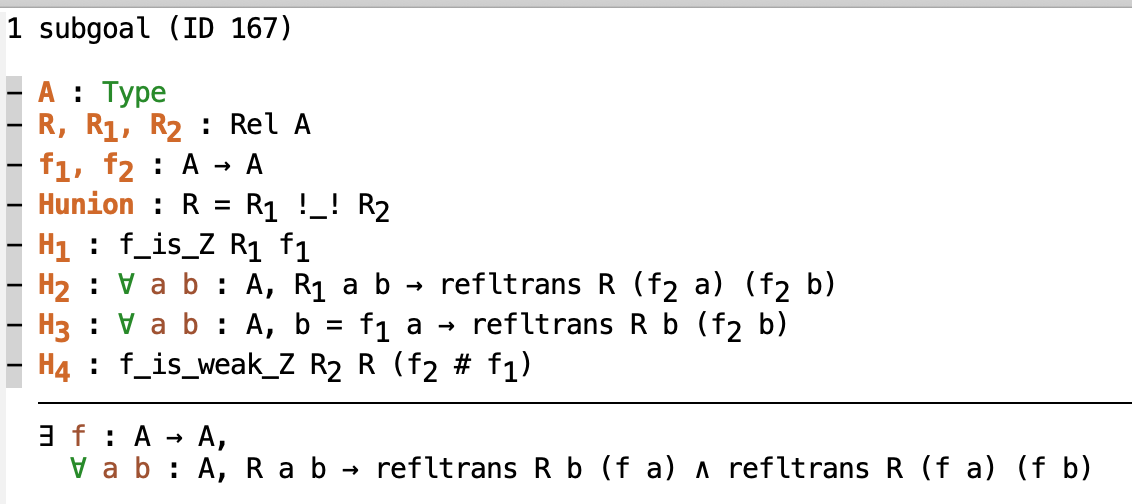
\includegraphics[scale=0.6]{fig8.png}


      Take the composition \coqdocvar{f2} \# \coqdocvar{f1} as \coqdocvar{f} as suggested by the above diagrams, and show that \coqdocvar{f2} \# \coqdocvar{f1} is Z. \begin{coqdoccode}
\coqdocemptyline
\coqdocindent{1.00em}
\coqdoctac{\ensuremath{\exists}} (\coqdocvar{f2} \coqref{ZtoConfl.:::x 'x23' x}{\coqdocnotation{\#}} \coqdocvar{f1}).\coqdoceol
\coqdocemptyline
\end{coqdoccode}
So, let \coqdocvar{a} and \coqdocvar{b} be elements of \coqdocvar{A}, and suppose that \coqdocvar{a} \coqdocvar{R}-reduces to \coqdocvar{b} in one step. Call \coqdocvar{HR} this hypothesis.  \begin{coqdoccode}
\coqdocemptyline
\coqdocindent{1.00em}
\coqdoctac{intros} \coqdocvar{a} \coqdocvar{b} \coqdocvar{HR}.\coqdoceol
\coqdocemptyline
\end{coqdoccode}
Since \coqdocvar{R} is the union of \coqdocvar{R1} and \coqdocvar{R2}, one has that \coqdocvar{a} reduces to \coqdocvar{b} in one step via either \coqdocvar{R1} or \coqdocvar{R2}.  \begin{coqdoccode}
\coqdocemptyline
\coqdocindent{1.00em}
\coqdoctac{inversion} \coqdocvar{Hunion}; \coqdoctac{subst}. \coqdoctac{clear} \coqdocvar{H}. \coqdoctac{inversion} \coqdocvar{HR}; \coqdoctac{subst}.\coqdoceol
\coqdocemptyline
\end{coqdoccode}
Firstly, suppose that \coqdocvar{a} \coqdocvar{R1}-reduces in one step to \coqdocvar{b}.  \begin{coqdoccode}
\coqdocemptyline
\coqdocindent{1.00em}
- \coqdoctac{split}.\coqdoceol
\coqdocemptyline
\end{coqdoccode}
In order to prove that \coqdocvar{b} R-reduces to ((\coqdocvar{f2} \# \coqdocvar{f1}) \coqdocvar{a}), we first need to show that \coqdocvar{b} \coqdocvar{R1}-reduces to (\coqdocvar{f1} \coqdocvar{a}) as shown in Figure \ref{fig:zcomp}. \begin{coqdoccode}
\coqdocemptyline
\coqdocindent{2.00em}
+ \coqdoctac{apply} \coqref{ZtoConfl.refltrans composition}{\coqdoclemma{refltrans\_composition}} \coqdockw{with} (\coqdocvar{f1} \coqdocvar{a}). \ensuremath{\times} \coqdoctac{apply} \coqdocvar{H1} \coqdoctac{in} \coqdocvar{H}. \coqdoctac{destruct} \coqdocvar{H}. \coqdoctac{apply} \coqref{ZtoConfl.refltrans union}{\coqdoclemma{refltrans\_union}}; \coqdoctac{assumption}.\coqdoceol
\coqdocemptyline
\end{coqdoccode}
The next step is then to prove that (\coqdocvar{f1} \coqdocvar{a}) \coqdocvar{R}-reduces to ((\coqdocvar{f2} \# \coqdocvar{f1}) \coqdocvar{a}), which is a direct consequence of \coqdocvar{H3}. \begin{coqdoccode}
\coqdocemptyline
\coqdocindent{3.00em}
\ensuremath{\times} \coqdoctac{apply} \coqdocvar{H3} \coqdockw{with} \coqdocvar{a}; \coqdoctac{reflexivity}.\coqdoceol
\coqdocemptyline
\end{coqdoccode}
The proof that ((\coqdocvar{f2} \# \coqdocvar{f1}) \coqdocvar{a}) \coqdocvar{R}-reduces to ((\coqdocvar{f2} \# \coqdocvar{f1}) \coqdocvar{b}) is more tricky. Initially, note that, since \coqdocvar{R1} \coqdocvar{a} \coqdocvar{b} then we get that \coqdocvar{refltrans} \coqdocvar{R1} (\coqdocvar{f1} \coqdocvar{a}) (\coqdocvar{f1} \coqdocvar{b}) by the Z property. \begin{coqdoccode}
\coqdocemptyline
\coqdocindent{2.00em}
+ \coqdoctac{apply} \coqdocvar{H1} \coqdoctac{in} \coqdocvar{H}. \coqdoctac{destruct} \coqdocvar{H}. \coqdoctac{clear} \coqdocvar{H} \coqdocvar{HR}. \coqdoctac{unfold} \coqref{ZtoConfl.comp}{\coqdocdefinition{comp}}.\coqdoceol
\coqdocemptyline
\end{coqdoccode}
Now, the goal can be obtained from \coqdocvar{H2} as long as \coqdocvar{R1} (\coqdocvar{f1} \coqdocvar{a}) (\coqdocvar{f1} \coqdocvar{b}), but we only have that \coqdocvar{refltrans} \coqdocvar{R1} (\coqdocvar{f1} \coqdocvar{a}) (\coqdocvar{f1} \coqdocvar{b}). Therefore, we use induction on this hypothesis. \begin{coqdoccode}
\coqdocemptyline
\coqdocindent{3.00em}
\coqdoctac{induction} \coqdocvar{H0}.\coqdoceol
\coqdocemptyline
\end{coqdoccode}
The reflexive case is trivial because \coqdocvar{a} and \coqdocvar{b} are equal.  \begin{coqdoccode}
\coqdocemptyline
\coqdocindent{3.00em}
\ensuremath{\times} \coqdoctac{apply} \coqref{ZtoConfl.refl}{\coqdocconstructor{refl}}.\coqdoceol
\coqdocemptyline
\end{coqdoccode}
In the transitive case, we have that (\coqdocvar{f1} \coqdocvar{a}) \coqdocvar{R1}-reduces to (\coqdocvar{f1} \coqdocvar{b}) in at least one step. The current proof context is as follows:


      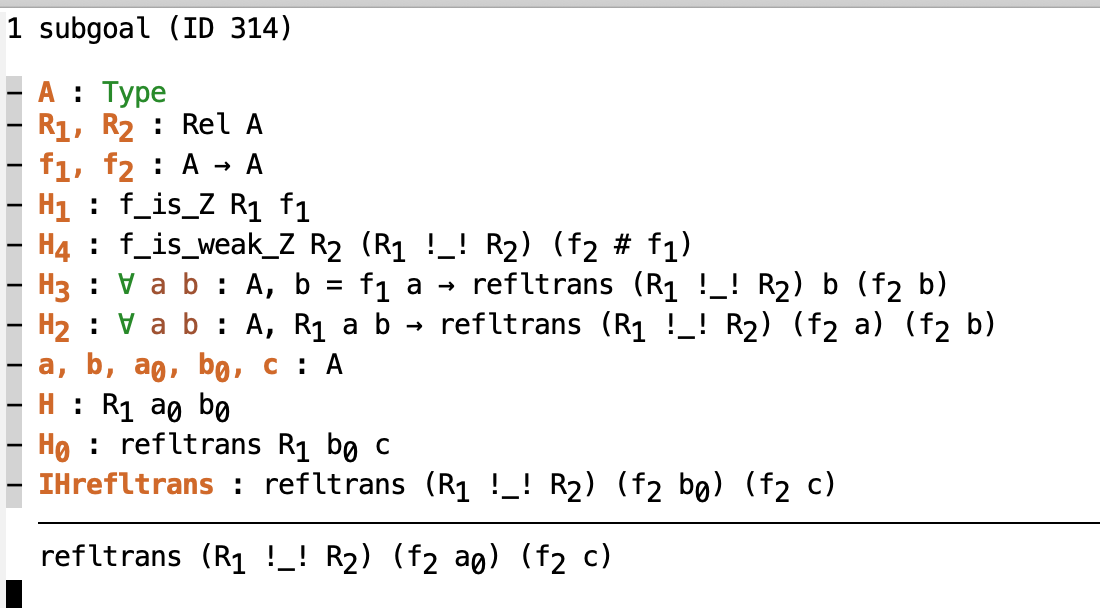
\includegraphics[scale=0.6]{fig9.png}


      Therefore, there exists some \coqdocvar{b0} such that \coqdocvar{R1} \coqdocvar{a0} \coqdocvar{b0} and \coqdocvar{refltrans} \coqdocvar{R1} \coqdocvar{b0} \coqdocvar{c} and we need to prove that \coqdocvar{refltrans} (\coqdocvar{R1} !\coqdocvar{\_}!  \coqdocvar{R2}) (\coqdocvar{f2} \coqdocvar{a0}) (\coqdocvar{f2} \coqdocvar{c}). This can be done in two steps by transitivity of \coqdocvar{refltrans} taking (\coqdocvar{f2} \coqdocvar{b0}) as the intermediary term. \begin{coqdoccode}
\coqdocemptyline
\coqdocindent{3.00em}
\ensuremath{\times} \coqdoctac{apply} \coqref{ZtoConfl.refltrans composition}{\coqdoclemma{refltrans\_composition}} \coqdockw{with} (\coqdocvar{f2} \coqdocvar{b0}).\coqdoceol
\coqdocemptyline
\end{coqdoccode}
The first subgoal is then \coqdocvar{refltrans} (\coqdocvar{R1} !\coqdocvar{\_}! \coqdocvar{R2}) (\coqdocvar{f2} \coqdocvar{a0}) (\coqdocvar{f2} \coqdocvar{b0}) that is proved by hypothesis \coqdocvar{H2}. \begin{coqdoccode}
\coqdocemptyline
\coqdocindent{4.00em}
** \coqdoctac{apply} \coqdocvar{H2}; \coqdoctac{assumption}.\coqdoceol
\coqdocemptyline
\end{coqdoccode}
And the second subgoal \coqdocvar{refltrans} (\coqdocvar{R1} !\coqdocvar{\_}! \coqdocvar{R2}) (\coqdocvar{f2} \coqdocvar{b0}) (\coqdocvar{f2} \coqdocvar{c}) is proved by the induction hypothesis. \begin{coqdoccode}
\coqdocemptyline
\coqdocindent{4.00em}
** \coqdoctac{assumption}.\coqdoceol
\coqdocemptyline
\end{coqdoccode}
Finally, when \coqdocvar{a} \coqdocvar{R2}-reduces in one step to \coqdocvar{b} one concludes the proof using the assumption that (\coqdocvar{f2} \# \coqdocvar{f1}) is weak Z. \begin{coqdoccode}
\coqdocemptyline
\coqdocindent{1.00em}
- \coqdoctac{apply} \coqdocvar{H4}; \coqdoctac{assumption}. \coqdockw{Qed}.\coqdoceol
\coqdocemptyline
\end{coqdoccode}
Now we can use the proofs of the theorems \coqdocvar{Z\_comp\_implies\_Z\_prop} and \coqdocvar{Z\_prop\_implies\_Confl} to conclude that compositional Z is a suficient condition for confluence. \begin{coqdoccode}
\coqdocemptyline
\coqdocnoindent
\coqdockw{Corollary} \coqdef{ZtoConfl.Z comp is Confl}{Z\_comp\_is\_Confl}{\coqdoclemma{Z\_comp\_is\_Confl}} \{\coqdocvar{A}\}: \coqdockw{\ensuremath{\forall}} (\coqdocvar{R}: \coqref{ZtoConfl.Rel}{\coqdocdefinition{Rel}} \coqdocvariable{A}), \coqref{ZtoConfl.Z comp}{\coqdocdefinition{Z\_comp}} \coqdocvariable{R} \coqexternalref{::type scope:x '->' x}{http://coq.inria.fr/distrib/V8.11.0/stdlib//Coq.Init.Logic}{\coqdocnotation{\ensuremath{\rightarrow}}} \coqref{ZtoConfl.Confl}{\coqdocdefinition{Confl}} \coqdocvariable{R}. \coqdockw{Proof}. \coqdoctac{intros} \coqdocvar{R} \coqdocvar{H}. \coqdoctac{apply} \coqref{ZtoConfl.Z comp implies Z prop}{\coqdoclemma{Z\_comp\_implies\_Z\_prop}} \coqdoctac{in} \coqdocvar{H}. \coqdoctac{apply} \coqref{ZtoConfl.Z prop implies Confl}{\coqdoclemma{Z\_prop\_implies\_Confl}}; \coqdoctac{assumption}. \coqdockw{Qed}.\coqdoceol
\coqdocemptyline
\end{coqdoccode}
Rewriting Systems with equations is another interesting and non-trivial topic \cite{winkler89,terese03}. The confluence of rewriting systems with an equivalence relation can also be proved by a variant of the compositional Z, known as Z property modulo~\cite{AK12b}.


    \begin{corollary}\cite{Nakazawa-Fujita2016}\label{cor:zcomp} Let $(A,\to)$ be an ARS such that $\to = \to_1 \cup \to_2$. If there exists mappings $f_1,f_2: A \to A$ such that \begin{enumerate} \item $a \to_1 b$ implies $f_1(a) = f_1(b)$ \item $a \tto_1 f_1(a), \forall a$ \item $a \tto f_2(a)$ holds for any $a\in Im(f_1)$ \item $f_2 \circ f_1$ is weakly Z for $\to_2$ by $\to$ \end{enumerate} then $f_2 \circ f_1$ is Z for $(A,\to)$, and hence $(A,\to)$ is confluent.  \end{corollary}


    We define the predicate \coqdocvar{Z\_comp\_eq} corresponding to the hypothesis of Corollary \ref{cor:zcomp}, and then we prove directly that if \coqdocvar{Z\_comp\_eq} holds for a relation \coqdocvar{R} then \coqdocvar{Zprop} \coqdocvar{R} also holds. This approach differs from \cite{Nakazawa-Fujita2016} that proves Corollary \ref{cor:zcomp} directly from Theorem \ref{thm:zcomp} \begin{coqdoccode}
\coqdocemptyline
\coqdocnoindent
\coqdockw{Definition} \coqdef{ZtoConfl.Z comp eq}{Z\_comp\_eq}{\coqdocdefinition{Z\_comp\_eq}} \{\coqdocvar{A}:\coqdockw{Type}\} (\coqdocvar{R} :\coqref{ZtoConfl.Rel}{\coqdocdefinition{Rel}} \coqdocvariable{A}) := \coqexternalref{::type scope:'exists' x '..' x ',' x}{http://coq.inria.fr/distrib/V8.11.0/stdlib//Coq.Init.Logic}{\coqdocnotation{\ensuremath{\exists}}} \coqexternalref{::type scope:'exists' x '..' x ',' x}{http://coq.inria.fr/distrib/V8.11.0/stdlib//Coq.Init.Logic}{\coqdocnotation{(}}\coqdocvar{R1} \coqdocvar{R2}: \coqref{ZtoConfl.Rel}{\coqdocdefinition{Rel}} \coqdocvariable{A}) (\coqdocvar{f1} \coqdocvar{f2}: \coqdocvariable{A} \coqexternalref{::type scope:x '->' x}{http://coq.inria.fr/distrib/V8.11.0/stdlib//Coq.Init.Logic}{\coqdocnotation{\ensuremath{\rightarrow}}} \coqdocvariable{A}\coqexternalref{::type scope:'exists' x '..' x ',' x}{http://coq.inria.fr/distrib/V8.11.0/stdlib//Coq.Init.Logic}{\coqdocnotation{),}} \coqdocvariable{R} \coqexternalref{::type scope:x '=' x}{http://coq.inria.fr/distrib/V8.11.0/stdlib//Coq.Init.Logic}{\coqdocnotation{=}} \coqexternalref{::type scope:x '=' x}{http://coq.inria.fr/distrib/V8.11.0/stdlib//Coq.Init.Logic}{\coqdocnotation{(}}\coqdocvariable{R1} \coqref{ZtoConfl.:::x '! !' x}{\coqdocnotation{!}}\coqref{ZtoConfl.:::x '! !' x}{\coqdocnotation{\_}}\coqref{ZtoConfl.:::x '! !' x}{\coqdocnotation{!}} \coqdocvariable{R2}\coqexternalref{::type scope:x '=' x}{http://coq.inria.fr/distrib/V8.11.0/stdlib//Coq.Init.Logic}{\coqdocnotation{)}} \coqexternalref{::type scope:x '/x5C' x}{http://coq.inria.fr/distrib/V8.11.0/stdlib//Coq.Init.Logic}{\coqdocnotation{\ensuremath{\land}}} \coqexternalref{::type scope:x '/x5C' x}{http://coq.inria.fr/distrib/V8.11.0/stdlib//Coq.Init.Logic}{\coqdocnotation{(}}\coqdockw{\ensuremath{\forall}} \coqdocvar{a} \coqdocvar{b}, \coqdocvariable{R1} \coqdocvariable{a} \coqdocvariable{b} \coqexternalref{::type scope:x '->' x}{http://coq.inria.fr/distrib/V8.11.0/stdlib//Coq.Init.Logic}{\coqdocnotation{\ensuremath{\rightarrow}}} \coqexternalref{::type scope:x '=' x}{http://coq.inria.fr/distrib/V8.11.0/stdlib//Coq.Init.Logic}{\coqdocnotation{(}}\coqdocvariable{f1} \coqdocvariable{a}\coqexternalref{::type scope:x '=' x}{http://coq.inria.fr/distrib/V8.11.0/stdlib//Coq.Init.Logic}{\coqdocnotation{)}} \coqexternalref{::type scope:x '=' x}{http://coq.inria.fr/distrib/V8.11.0/stdlib//Coq.Init.Logic}{\coqdocnotation{=}} \coqexternalref{::type scope:x '=' x}{http://coq.inria.fr/distrib/V8.11.0/stdlib//Coq.Init.Logic}{\coqdocnotation{(}}\coqdocvariable{f1} \coqdocvariable{b}\coqexternalref{::type scope:x '=' x}{http://coq.inria.fr/distrib/V8.11.0/stdlib//Coq.Init.Logic}{\coqdocnotation{)}}\coqexternalref{::type scope:x '/x5C' x}{http://coq.inria.fr/distrib/V8.11.0/stdlib//Coq.Init.Logic}{\coqdocnotation{)}} \coqexternalref{::type scope:x '/x5C' x}{http://coq.inria.fr/distrib/V8.11.0/stdlib//Coq.Init.Logic}{\coqdocnotation{\ensuremath{\land}}} \coqexternalref{::type scope:x '/x5C' x}{http://coq.inria.fr/distrib/V8.11.0/stdlib//Coq.Init.Logic}{\coqdocnotation{(}}\coqdockw{\ensuremath{\forall}} \coqdocvar{a}, (\coqref{ZtoConfl.refltrans}{\coqdocinductive{refltrans}} \coqdocvariable{R1}) \coqdocvariable{a} (\coqdocvariable{f1} \coqdocvariable{a})\coqexternalref{::type scope:x '/x5C' x}{http://coq.inria.fr/distrib/V8.11.0/stdlib//Coq.Init.Logic}{\coqdocnotation{)}} \coqexternalref{::type scope:x '/x5C' x}{http://coq.inria.fr/distrib/V8.11.0/stdlib//Coq.Init.Logic}{\coqdocnotation{\ensuremath{\land}}} \coqexternalref{::type scope:x '/x5C' x}{http://coq.inria.fr/distrib/V8.11.0/stdlib//Coq.Init.Logic}{\coqdocnotation{(}}\coqdockw{\ensuremath{\forall}} \coqdocvar{b} \coqdocvar{a}, \coqdocvariable{a} \coqexternalref{::type scope:x '=' x}{http://coq.inria.fr/distrib/V8.11.0/stdlib//Coq.Init.Logic}{\coqdocnotation{=}} \coqdocvariable{f1} \coqdocvariable{b} \coqexternalref{::type scope:x '->' x}{http://coq.inria.fr/distrib/V8.11.0/stdlib//Coq.Init.Logic}{\coqdocnotation{\ensuremath{\rightarrow}}} (\coqref{ZtoConfl.refltrans}{\coqdocinductive{refltrans}} \coqdocvariable{R}) \coqdocvariable{a} (\coqdocvariable{f2} \coqdocvariable{a})\coqexternalref{::type scope:x '/x5C' x}{http://coq.inria.fr/distrib/V8.11.0/stdlib//Coq.Init.Logic}{\coqdocnotation{)}} \coqexternalref{::type scope:x '/x5C' x}{http://coq.inria.fr/distrib/V8.11.0/stdlib//Coq.Init.Logic}{\coqdocnotation{\ensuremath{\land}}} \coqexternalref{::type scope:x '/x5C' x}{http://coq.inria.fr/distrib/V8.11.0/stdlib//Coq.Init.Logic}{\coqdocnotation{(}}\coqref{ZtoConfl.f is weak Z}{\coqdocdefinition{f\_is\_weak\_Z}} \coqdocvariable{R2} \coqdocvariable{R} (\coqdocvariable{f2} \coqref{ZtoConfl.:::x 'x23' x}{\coqdocnotation{\#}} \coqdocvariable{f1})\coqexternalref{::type scope:x '/x5C' x}{http://coq.inria.fr/distrib/V8.11.0/stdlib//Coq.Init.Logic}{\coqdocnotation{)}}.\coqdoceol
\coqdocemptyline
\coqdocnoindent
\coqdockw{Lemma} \coqdef{ZtoConfl.Z comp eq implies Z prop}{Z\_comp\_eq\_implies\_Z\_prop}{\coqdoclemma{Z\_comp\_eq\_implies\_Z\_prop}} \{\coqdocvar{A}:\coqdockw{Type}\}: \coqdockw{\ensuremath{\forall}} (\coqdocvar{R} : \coqref{ZtoConfl.Rel}{\coqdocdefinition{Rel}} \coqdocvariable{A}), \coqref{ZtoConfl.Z comp eq}{\coqdocdefinition{Z\_comp\_eq}} \coqdocvariable{R} \coqexternalref{::type scope:x '->' x}{http://coq.inria.fr/distrib/V8.11.0/stdlib//Coq.Init.Logic}{\coqdocnotation{\ensuremath{\rightarrow}}} \coqref{ZtoConfl.Z prop}{\coqdocdefinition{Z\_prop}} \coqdocvariable{R}. \coqdockw{Proof}.\coqdoceol
\coqdocemptyline
\end{coqdoccode}
Let \coqdocvar{R} be a relation and suppose that \coqdocvar{R} satisfies the predicate \coqdocvar{Z\_comp\_eq}. \begin{coqdoccode}
\coqdocemptyline
\coqdocindent{1.00em}
\coqdoctac{intros} \coqdocvar{R} \coqdocvar{Heq}. \coqdoctac{unfold} \coqref{ZtoConfl.Z comp eq}{\coqdocdefinition{Z\_comp\_eq}} \coqdoctac{in} \coqdocvar{Heq}.\coqdoceol
\coqdocemptyline
\end{coqdoccode}
Call \coqdocvar{Hi} the \coqdocvar{i}th hypothesis as in \ref{cor:zcomp}.  \begin{coqdoccode}
\coqdocemptyline
\coqdocindent{1.00em}
\coqdoctac{destruct} \coqdocvar{Heq} \coqdockw{as} [\coqdocvar{R1} [\coqdocvar{R2} [\coqdocvar{f1} [\coqdocvar{f2} [\coqdocvar{Hunion} [\coqdocvar{H1} [\coqdocvar{H2} [\coqdocvar{H3} \coqdocvar{H4}]]]]]]]].\coqdoceol
\coqdocemptyline
\end{coqdoccode}
From the definition of the predicate \coqdocvar{Z\_prop}, we need to find a map, say \coqdocvar{f} that is Z. Let (\coqdocvar{f2} \# \coqdocvar{f1}) be such map.  \begin{coqdoccode}
\coqdocemptyline
\coqdocindent{1.00em}
\coqdoctac{unfold} \coqref{ZtoConfl.Z prop}{\coqdocdefinition{Z\_prop}}. \coqdoctac{\ensuremath{\exists}} (\coqdocvar{f2} \coqref{ZtoConfl.:::x 'x23' x}{\coqdocnotation{\#}} \coqdocvar{f1}).\coqdoceol
\coqdocemptyline
\end{coqdoccode}
In order to prove that (\coqdocvar{f2} \# \coqdocvar{f1}) is Z, let \coqdocvar{a} and \coqdocvar{b} be arbitrary elements of type \coqdocvar{A}, and \coqdocvar{Hab} be the hypothesis that \coqdocvar{a} \coqdocvar{R}-reduces in one step to \coqdocvar{b}.  \begin{coqdoccode}
\coqdocemptyline
\coqdocindent{1.00em}
\coqdoctac{intros} \coqdocvar{a} \coqdocvar{b} \coqdocvar{Hab}.\coqdoceol
\coqdocemptyline
\end{coqdoccode}
Since \coqdocvar{a} \coqdocvar{R}-reduces in one step to \coqdocvar{b} and \coqdocvar{R} is the union of the relations \coqdocvar{R1} and \coqdocvar{R2} then we consider two cases: \begin{coqdoccode}
\coqdocemptyline
\coqdocindent{1.00em}
\coqdoctac{inversion} \coqdocvar{Hunion}; \coqdoctac{subst}; \coqdoctac{clear} \coqdocvar{H}. \coqdoctac{inversion} \coqdocvar{Hab}; \coqdoctac{subst}; \coqdoctac{clear} \coqdocvar{Hab}.\coqdoceol
\coqdocemptyline
\end{coqdoccode}
The first case is when \coqdocvar{a} \coqdocvar{R1}-reduces in one step to \coqdocvar{b}. \begin{coqdoccode}
\coqdocemptyline
\coqdocindent{1.00em}
- \coqdoctac{unfold} \coqref{ZtoConfl.comp}{\coqdocdefinition{comp}}; \coqdoctac{split}.\coqdoceol
\coqdocemptyline
\end{coqdoccode}
This is equivalent to say that \coqdocvar{f2} \# \coqdocvar{f1} is weak Z for \coqdocvar{R1} by \coqdocvar{R1} !\coqdocvar{\_}! \coqdocvar{R2}. Therefore, we first prove that \coqdocvar{refltrans} (\coqdocvar{R1} !\coqdocvar{\_}! \coqdocvar{R2}) \coqdocvar{b} (\coqdocvar{f2} (\coqdocvar{f1} \coqdocvar{a})), which can be reduced to \coqdocvar{refltrans} (\coqdocvar{R1} !\coqdocvar{\_}! \coqdocvar{R2}) \coqdocvar{b} (\coqdocvar{f1} \coqdocvar{b}) and \coqdocvar{refltrans} (\coqdocvar{R1} !\coqdocvar{\_}! \coqdocvar{R2}) (\coqdocvar{f1} \coqdocvar{b}) (\coqdocvar{f2} (\coqdocvar{f1} \coqdocvar{a})) by the transitivity of \coqdocvar{refltrans}. \begin{coqdoccode}
\coqdocemptyline
\coqdocindent{2.00em}
+ \coqdoctac{apply} \coqref{ZtoConfl.refltrans composition}{\coqdoclemma{refltrans\_composition}} \coqdockw{with} (\coqdocvar{f1} \coqdocvar{b}).\coqdoceol
\coqdocemptyline
\end{coqdoccode}
From hypothesis \coqdocvar{H2}, we know that \coqdocvar{refltrans} \coqdocvar{R1} \coqdocvar{a} (\coqdocvar{f1} \coqdocvar{a}) for all \coqdocvar{a}, and hence \coqdocvar{refltrans} (\coqdocvar{R1} !\coqdocvar{\_}! \coqdocvar{R2}) \coqdocvar{a} (\coqdocvar{f1} \coqdocvar{a}) and we conclude.\begin{coqdoccode}
\coqdocemptyline
\coqdocindent{3.00em}
\ensuremath{\times} \coqdoctac{apply} \coqref{ZtoConfl.refltrans union}{\coqdoclemma{refltrans\_union}}. \coqdoctac{apply} \coqdocvar{H2}.\coqdoceol
\coqdocemptyline
\end{coqdoccode}
The proof that \coqdocvar{refltrans} (\coqdocvar{R1} !\coqdocvar{\_}! \coqdocvar{R2}) (\coqdocvar{f1} \coqdocvar{b}) (\coqdocvar{f2} (\coqdocvar{f1} \coqdocvar{a})) is exactly the content of hypothesis \coqdocvar{H3}.  \begin{coqdoccode}
\coqdocemptyline
\coqdocindent{3.00em}
\ensuremath{\times} \coqdoctac{apply} \coqdocvar{H1} \coqdoctac{in} \coqdocvar{H}. \coqdoctac{rewrite} \coqdocvar{H}. \coqdoctac{apply} \coqdocvar{H3} \coqdockw{with} \coqdocvar{b}; \coqdoctac{reflexivity}.\coqdoceol
\coqdocemptyline
\end{coqdoccode}
The proof that \coqdocvar{refltrans} (\coqdocvar{R1} !\coqdocvar{\_}! \coqdocvar{R2}) (\coqdocvar{f2} (\coqdocvar{f1} \coqdocvar{a})) (\coqdocvar{f2} (\coqdocvar{f1} \coqdocvar{b})) is done using the reflexivity of \coqdocvar{refltrans} because  (\coqdocvar{f2} (\coqdocvar{f1} \coqdocvar{a})) = (\coqdocvar{f2} (\coqdocvar{f1} \coqdocvar{b})) by hypothesis \coqdocvar{H1}. \begin{coqdoccode}
\coqdocemptyline
\coqdocindent{2.00em}
+ \coqdoctac{apply} \coqdocvar{H1} \coqdoctac{in} \coqdocvar{H}. \coqdoctac{rewrite} \coqdocvar{H}. \coqdoctac{apply} \coqref{ZtoConfl.refl}{\coqdocconstructor{refl}}.\coqdoceol
\coqdocemptyline
\end{coqdoccode}
When \coqdocvar{a} \coqdocvar{R2}-reduces in one step to \coqdocvar{b} then we are done by hypothesis \coqdocvar{H4}. \begin{coqdoccode}
\coqdocemptyline
\coqdocindent{1.00em}
- \coqdoctac{apply} \coqdocvar{H4}; \coqdoctac{assumption}. \coqdockw{Qed}.\coqdoceol
\coqdocemptyline
\end{coqdoccode}
